\documentclass{beamer}
\useoutertheme[progressbar=frametitle]{metropolis}
\useinnertheme{metropolis}
\definecolor{nabgray}{rgb}{0.6,0.59,0.61}
\usecolortheme[named=nabgray]{structure}

\usepackage{tikz}
\usepackage[utf8]{inputenc}
\usepackage[english]{babel}

\usepackage{smartdiagram}
\usepackage{qtree}
\usepackage{verbatim}
\usepackage{svg}
\usepackage{graphicx}
\usepackage{color}
\definecolor{lightgray}{rgb}{0.95, 0.95, 0.95}
\definecolor{darkgray}{rgb}{0.4, 0.4, 0.4}
%\definecolor{purple}{rgb}{0.65, 0.12, 0.82}
\definecolor{editorGray}{rgb}{0.95, 0.95, 0.95}
\definecolor{editorOcher}{rgb}{1, 0.5, 0} % #FF7F00 -> rgb(239, 169, 0)
\definecolor{editorGreen}{rgb}{0, 0.5, 0} % #007C00 -> rgb(0, 124, 0)
\definecolor{orange}{rgb}{1,0.45,0.13}		
\definecolor{olive}{rgb}{0.17,0.59,0.20}
\definecolor{brown}{rgb}{0.69,0.31,0.31}
\definecolor{purple}{rgb}{0.38,0.18,0.81}
\definecolor{lightblue}{rgb}{0.1,0.57,0.7}
\definecolor{lightred}{rgb}{1,0.4,0.5}
\usepackage{upquote}
\usepackage{listings}
\lstset{language=java,
	basicstyle=\footnotesize\ttfamily,
	keywordstyle=\footnotesize\color{blue}\ttfamily,
}


\usebackgroundtemplate%
{%
	
\includegraphics[width=\paperwidth]{Images/Contenido}%
}


\title{Eclipse MicroProfile Metrics: Practical use cases}
\author{Jorge Cajas - José Diaz - Víctor Orozco}
\institute{GuateJUG - PeruJUG}
\date{\today}

\begin{document}

\frame{\titlepage}

\begin{frame}{Overview}
\tableofcontents
\end{frame} 


\begin{frame}{Víctor Orozco}
\begin{columns}[T] % contents are top vertically aligned
	\begin{column}[T]{6cm} % each column can also be its own environment
		\begin{itemize}
			\item I like Java EE
			\item CTO@Nabenik
			\item \href{https://twitter.com/tuxtor}{@tuxtor}
			\item \href{http://vorozco.com}{http://vorozco.com}
			\item \href{http://tuxtor.shekalug.org}{http://tuxtor.shekalug.org} 
		\end{itemize}
	\end{column}
	\begin{column}[T]{4cm} % alternative top-align that's better for graphics
		\begin{figure}
			\centering
			
\includegraphics[width=\linewidth]{Images/logos}
		\end{figure}
	\end{column}
\end{columns}
\end{frame}

\begin{frame}{Jorge Cajas}
\begin{columns}[T] % contents are top vertically aligned
	\begin{column}[T]{5cm} % each column can also be its own environment
		\begin{itemize}
			\item JUG Leader
		\end{itemize}
	\end{column}
	\begin{column}[T]{5cm} % alternative top-align that's better for graphics
		\begin{figure}
			\centering
			
\includegraphics[width=0.6\linewidth]{Images/logos}
		\end{figure}
		
	\end{column}
\end{columns}
\end{frame}

\begin{frame}{José Díaz}
\begin{columns}[T] % contents are top vertically aligned
	\begin{column}[T]{5cm} % each column can also be its own environment
		\begin{itemize}
			\item JUG Leader
		\end{itemize}
	\end{column}
	\begin{column}[T]{5cm} % alternative top-align that's better for graphics
		\begin{figure}
			\centering
			
\includegraphics[width=0.6\linewidth]{Images/logos}
		\end{figure}
		
	\end{column}
\end{columns}
\end{frame}

\section{Why Metrics?}
\begin{frame}{Why Metrics?}
\Large Do I need metrics?
\begin{figure}
	\centering
	
\includegraphics[width=0.6\linewidth]{Images/dukewhy}
\end{figure}
\end{frame}


\begin{frame}{Why Metrics?}

\begin{figure}
	\centering
	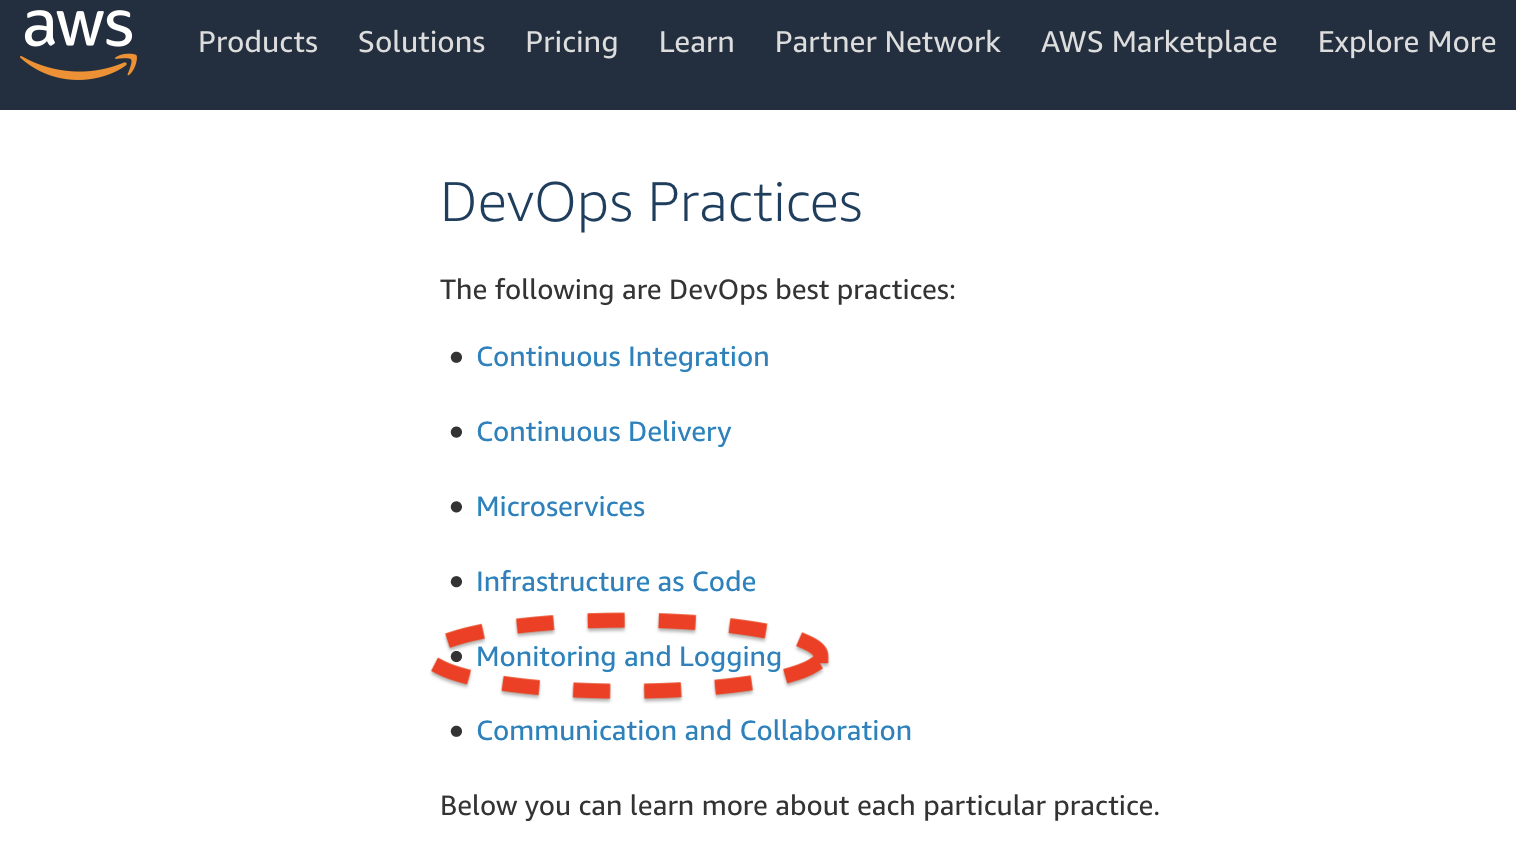
\includegraphics[width=\linewidth]{Images/amazondevops}
\end{figure}
\end{frame}

\begin{frame}{Why Metrics?}
\Large What about non-DevOps?
\begin{figure}
	\centering
	
\includegraphics[width=0.6\linewidth]{Images/dukewhy}
\end{figure}
\end{frame}

\section{Monoliths}
\begin{frame}{Metrics in Java Monoliths}
\begin{columns}[T] % contents are top vertically aligned
	\begin{column}[T]{3cm} % each column can also be its own environment
		\begin{itemize}
			\item Long running JVM
			\item Scale as . . . more long running JVMs
			\item Ideally never rebooted
		\end{itemize}
	\end{column}
	\begin{column}[T]{7cm} % alternative top-align that's better for graphics
		\begin{figure}
			\centering
			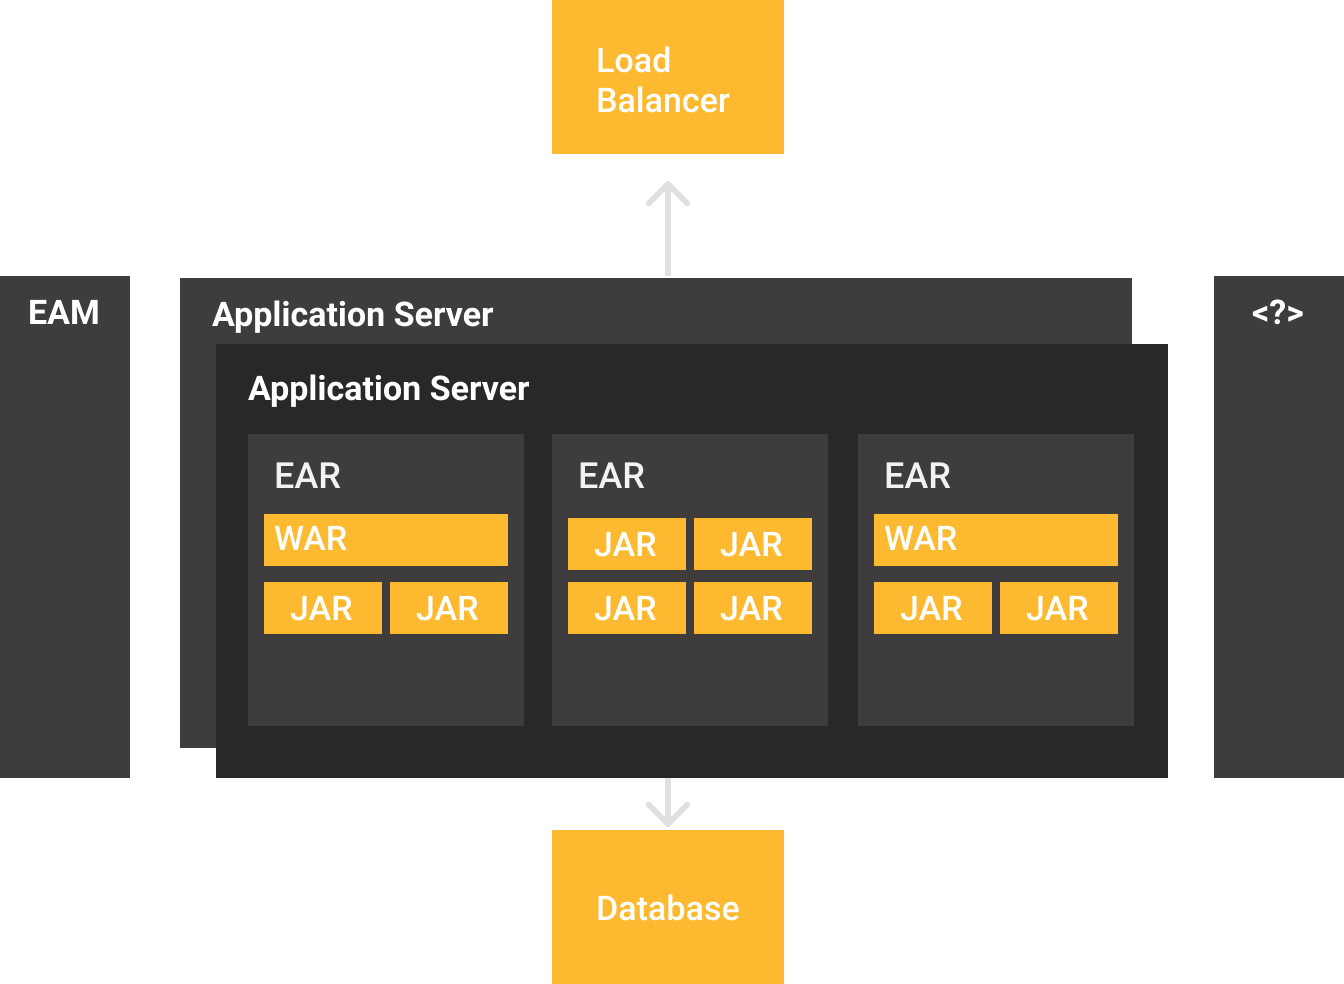
\includegraphics[width=\linewidth]{Images/monolitos}
		\end{figure}
		
	\end{column}
\end{columns}
\end{frame}

\begin{frame}{Metrics in Java Monoliths}
\begin{columns}[T] % contents are top vertically aligned
	\begin{column}[T]{3cm} % each column can also be its own environment
		\begin{enumerate}
			\item Telemetry Vendor APIs (Glassfish Metrics)
			\item JMX  (VisualVM, Mission Control)
			\item Shell wranglers + Logs
		\end{enumerate}
	\end{column}
	\begin{column}[T]{7cm} % alternative top-align that's better for graphics
		\begin{figure}
			\centering
			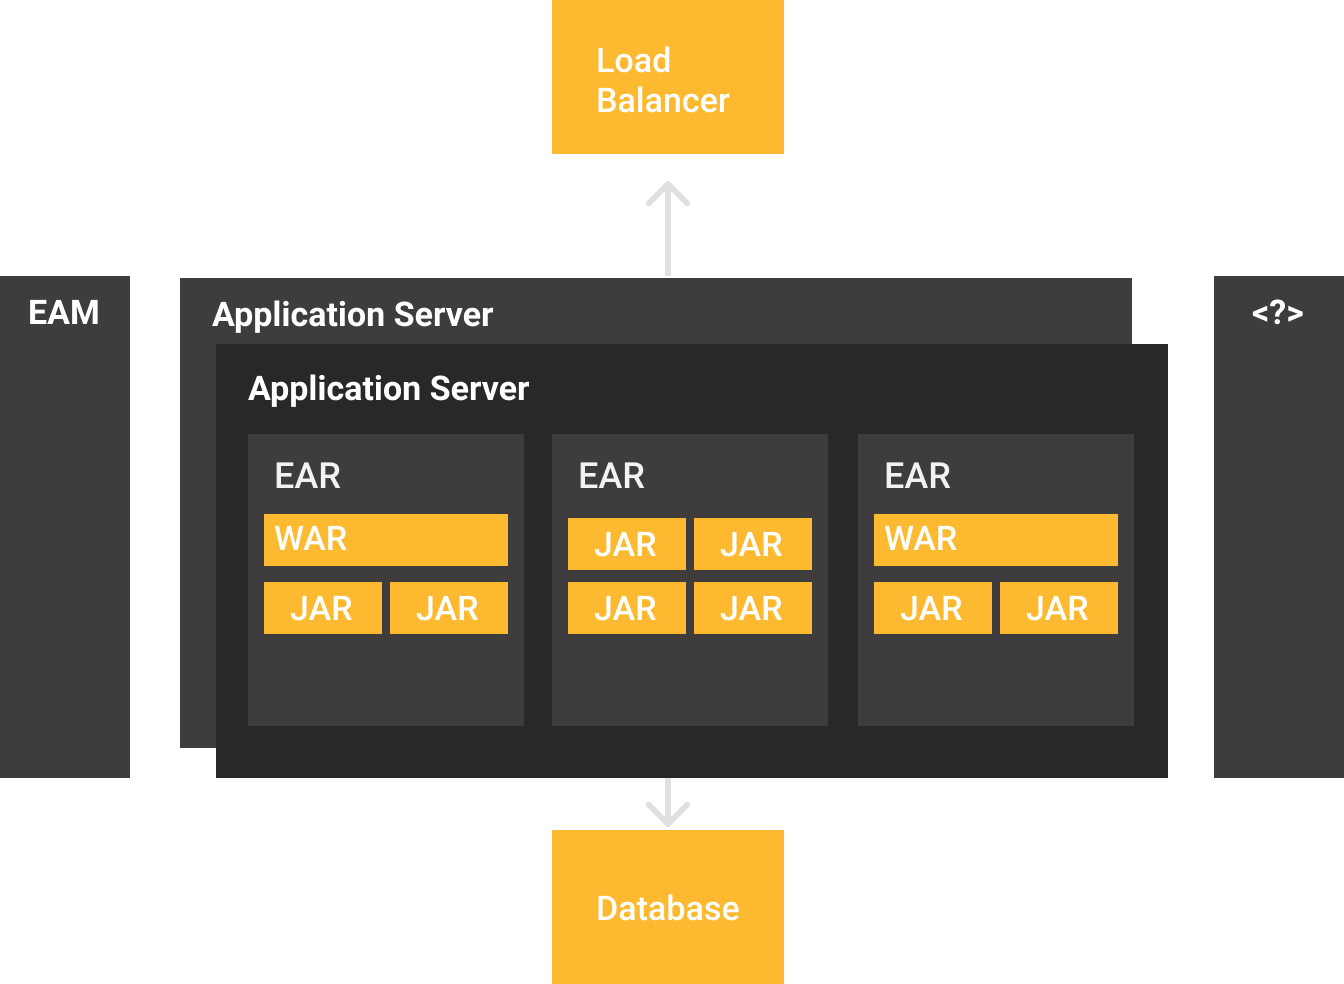
\includegraphics[width=\linewidth]{Images/monolitos}
		\end{figure}
		
	\end{column}
\end{columns}
\end{frame}

\begin{frame}{Metrics in Java Monoliths}
\Large How do I choose between JMX or a telemetry API? How do I get access to JMX if I´m using PaaS?
\begin{figure}
	\centering
	
\includegraphics[width=0.6\linewidth]{Images/dukewhy}
\end{figure}
\end{frame}


\section{Reactive applications}
\begin{frame}{Reactive applications}
Reactive often means Microservices
\begin{figure}
	\centering
	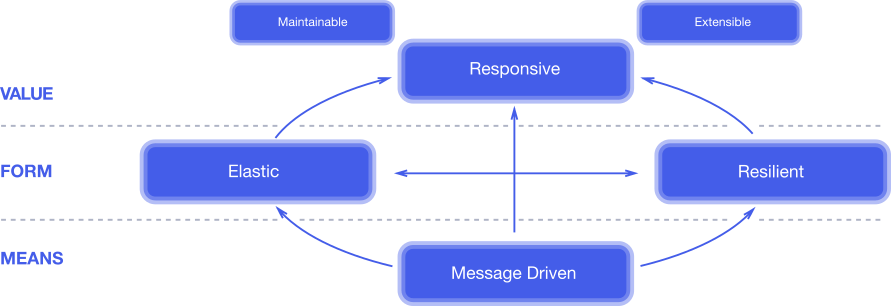
\includegraphics[width=\linewidth]{Images/reactive-traits}
\end{figure}
Key concept: Non-long running JVM
\end{frame}


\begin{frame}{Metrics in Microservices}
\begin{columns}[T] % contents are top vertically aligned
	\begin{column}[T]{3cm} % each column can also be its own environment
		\begin{itemize}
			\item Short lived JVMs
			\item Orchestrated through Swarm/Kubernetes
			\item Provisioned as needed
		\end{itemize}
	\end{column}
	\begin{column}[T]{7cm} % alternative top-align that's better for graphics
		\begin{figure}
			\centering
			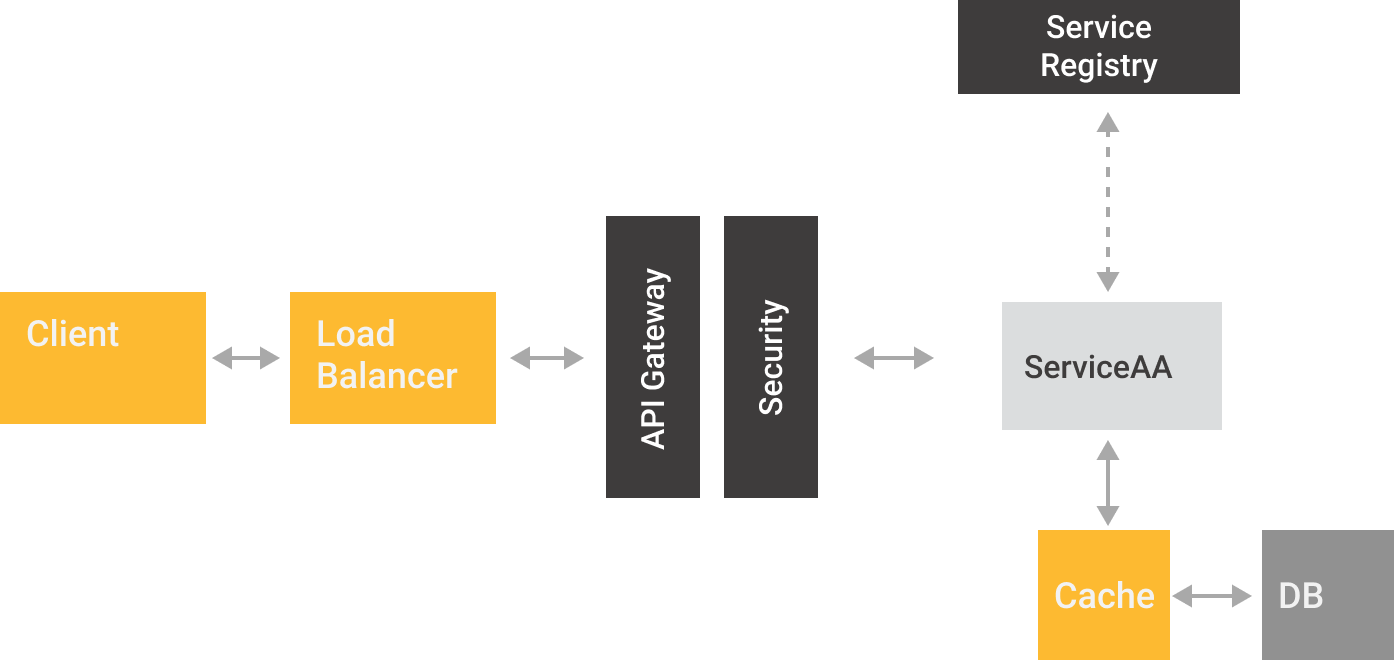
\includegraphics[width=\linewidth]{Images/microservicios}
		\end{figure}
		
	\end{column}
\end{columns}
\end{frame}

\begin{frame}{Metrics in Microservices}
\begin{columns}[T] % contents are top vertically aligned
	\begin{column}[T]{3cm} % each column can also be its own environment
		\begin{itemize}
			\item JVM over CaaS over PaaS
			\item Dynamic and ever-changing addresses and ports
			\item Logs inside the container
		\end{itemize}
	\end{column}
	\begin{column}[T]{7cm} % alternative top-align that's better for graphics
		\begin{figure}
			\centering
			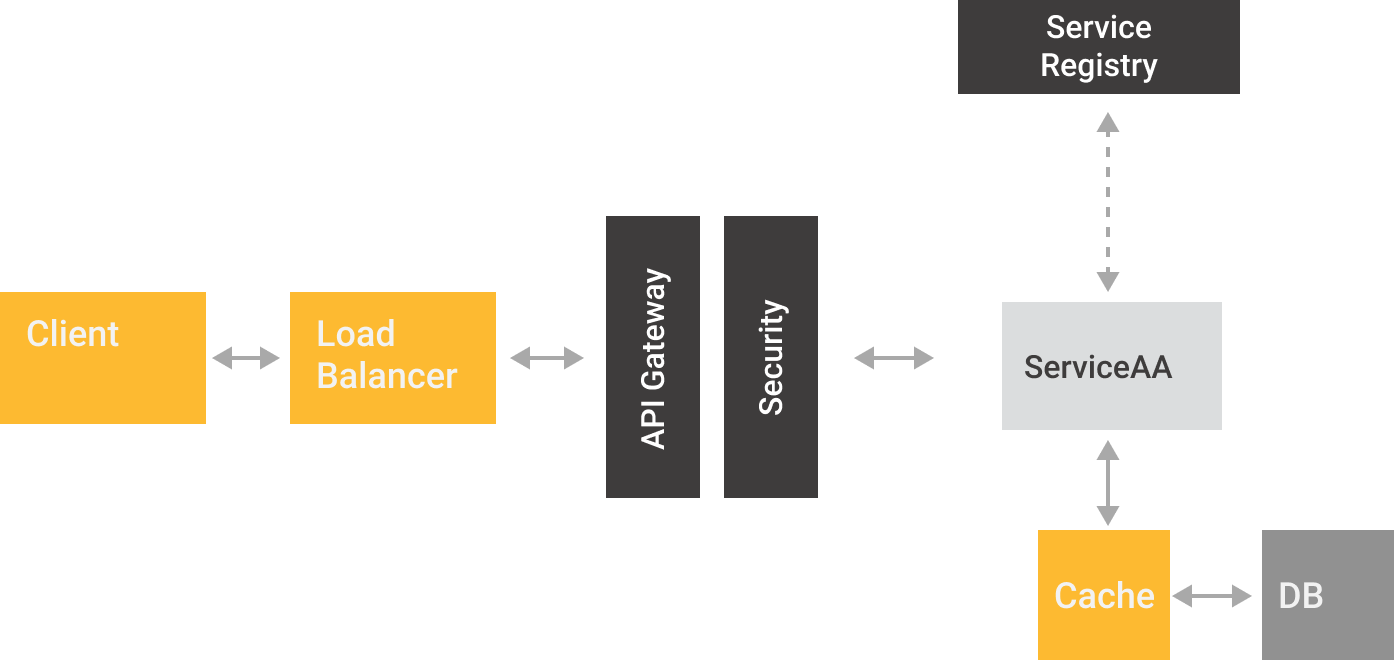
\includegraphics[width=\linewidth]{Images/microservicios}
		\end{figure}
		
	\end{column}
\end{columns}
\end{frame}

\section{Eclipse MicroProfile}

\begin{frame}{Eclipse MicroProfile}
	\begin{figure}
		\centering
		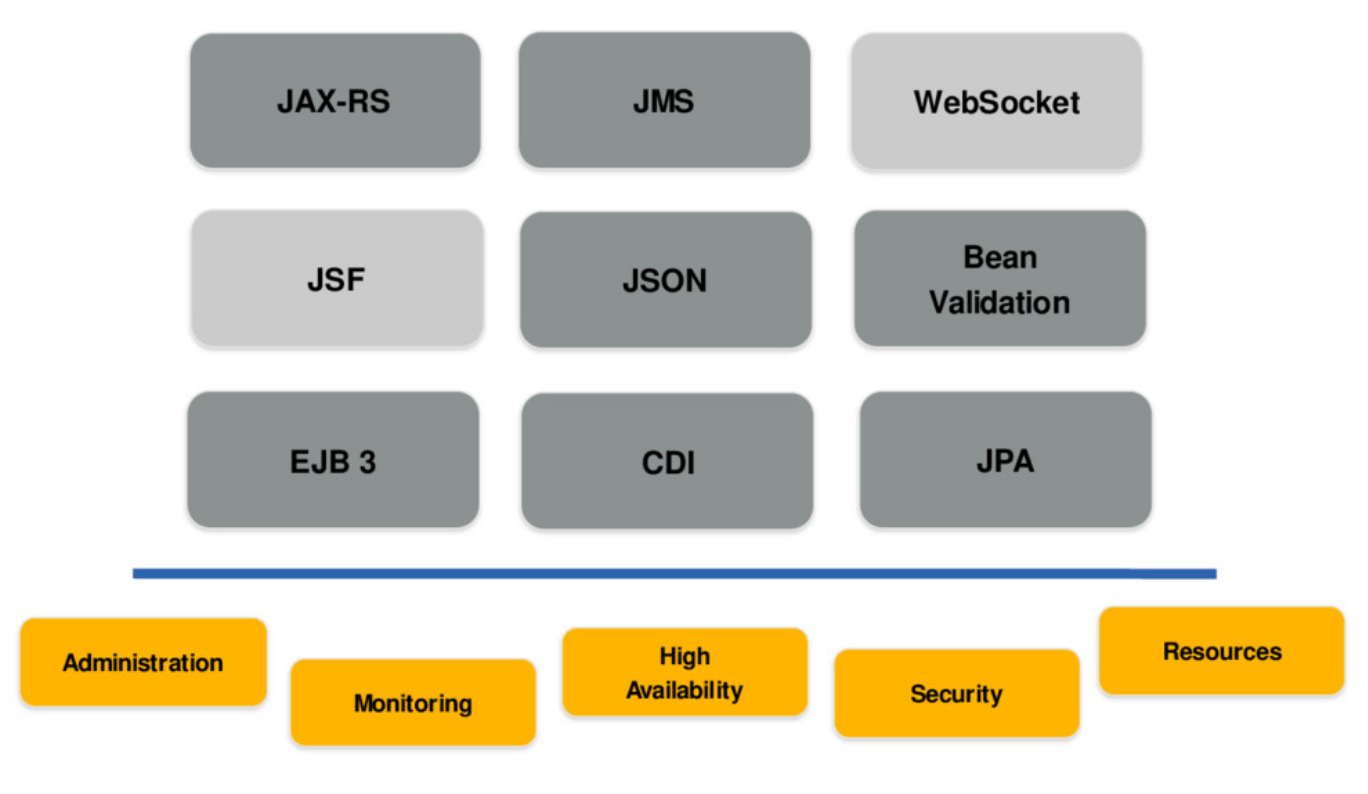
\includegraphics[width=\linewidth]{Images/javaeemicropancake}
		\caption{Credits: Reza Rahman}
	\end{figure}
\end{frame}

\begin{frame}{Eclipse MicroProfile}
\begin{figure}
	\centering
	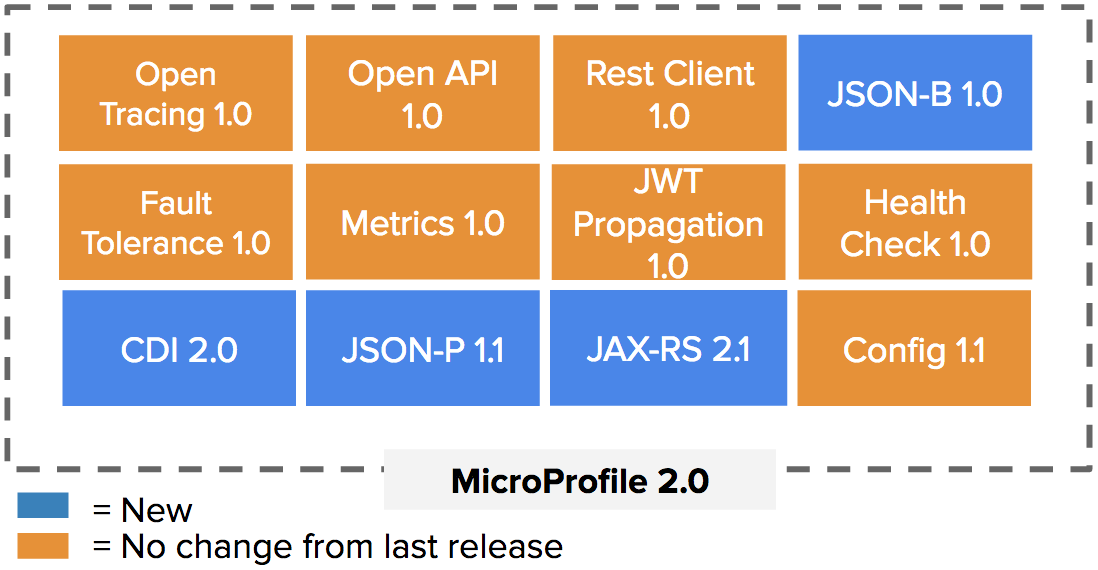
\includegraphics[width=\linewidth]{Images/mp5}
\end{figure}
\end{frame}

\begin{frame}[fragile]{Eclipse MicroProfile on Payara 5}
\begin{lstlisting}
<dependency>
	<groupId>org.eclipse.microprofile</groupId>
	<artifactId>microprofile</artifactId>
	<type>pom</type>
	<version>2.0.1</version>
	<scope>provided</scope>
</dependency>
\end{lstlisting}
\end{frame}




\begin{frame}{EE + MicroProfile  - Demo}
\huge Java 8, JAX-RS, CDI, EJB, Microprofile

\normalsize  \url{https://github.com/tuxtor/payara-demo}\\
\normalsize  \url{https://github.com/tuxtor/omdb-demo}
\end{frame}

\begin{frame}{Payara Micro - Traditional Java EE}
Take for granted
\begin{columns}[T] % contents are top vertically aligned
\begin{column}[T]{3cm} % each column can also be its own environment
\begin{itemize}
\item EJB
\item \textbf{JTA}
\item JAX-RS
\item CDI
\end{itemize}
\end{column}
\begin{column}[T]{7cm} % alternative top-align that's better for graphics
\begin{figure}
\centering
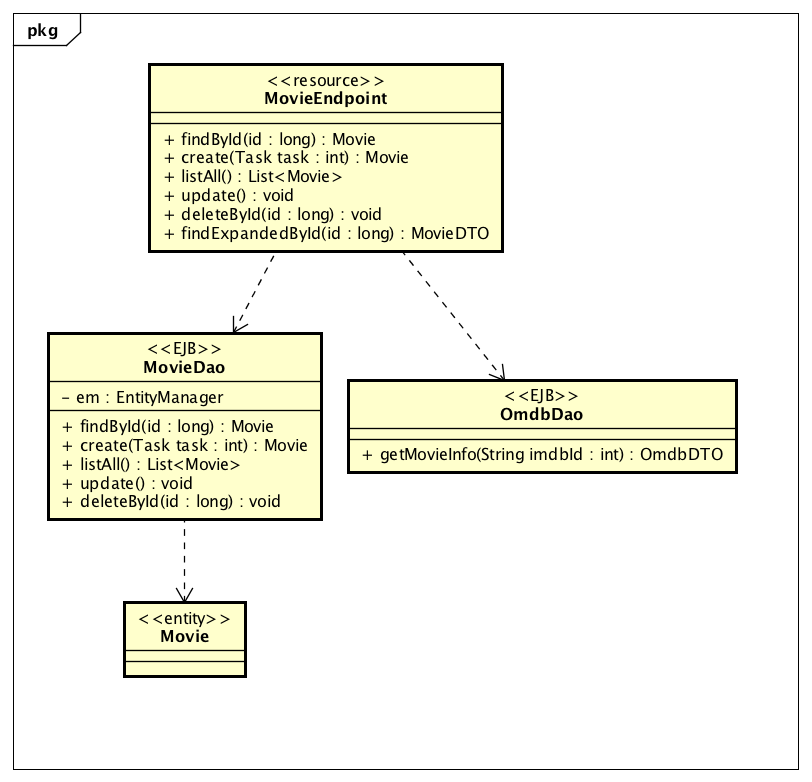
\includegraphics[width=\linewidth]{Images/democlass}
\end{figure}
\end{column}
\end{columns}
\end{frame}

\begin{frame}{EE + MicroProfile - Demo}
\footnotesize MicroProfile: JAX-RS, CDI (Per service), Config, Fault Tolerance, Metrics\\
Payara Micro: EJB, JTA (Per service)\\
External: Location, Deployment, Orchestation, Balancing, Consistency, Patterns
\begin{figure}
\centering
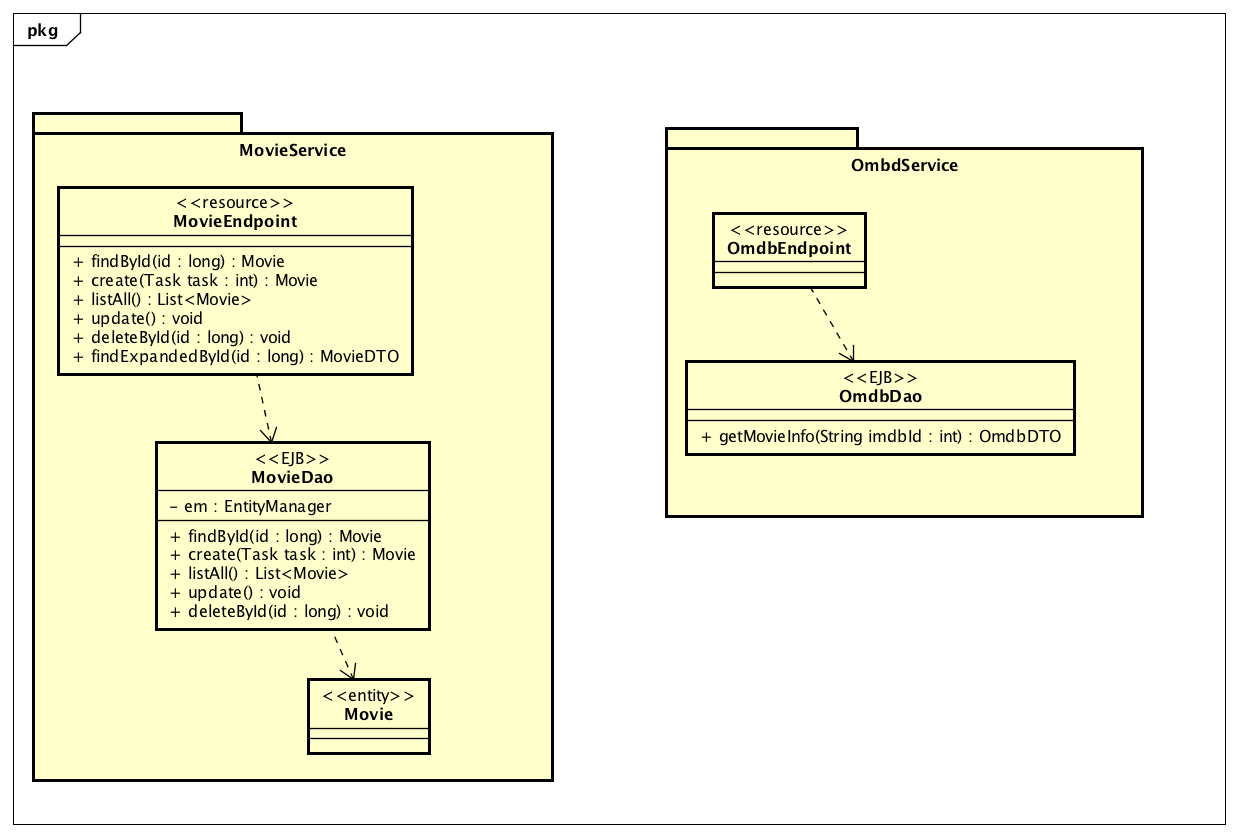
\includegraphics[width=0.95\linewidth]{Images/demomicro}
\end{figure}

\end{frame}

\begin{frame}[fragile]{Config}
\begin{lstlisting}
@Inject
@ConfigProperty(name = "omdbservice.url")
String omdbDaemonServiceUrl;
\end{lstlisting}
\end{frame}

\begin{frame}{Fault tolerance}

\begin{itemize}
\item Circuit Breaker
\item Bulkhead
\item Fallback
\item Retry
\item Timeout
\end{itemize}

\end{frame}


\begin{frame}[fragile]{Fault tolerance - Fallback, Timeout}
\begin{lstlisting}
@GET
@Path("/{id:[a-z]*[0-9][0-9]*}")
@Fallback(fallbackMethod = "findByIdFallBack")
@Timeout(TIMEOUT)
public Response findById(@PathParam("id") 
final String imdbId) {
...
}

public Response findByIdFallBack(@PathParam("id") 
final String imdbId) {
...
}
\end{lstlisting}
\end{frame}


\begin{frame}{Metrics}

Where
\begin{itemize}
	\item JSON or OpenMetrics (Prometheus)
	\item Vendor
	\item Base
	\item Application
\end{itemize}

How
\begin{itemize}
	\item Counted
	\item Gauge
	\item Metered
	\item Timed
	\item Histogram
\end{itemize}

\end{frame}


\section{Practical Use Cases}


\begin{frame}{Case 0 - Metrics for microservices}

\begin{enumerate}
	\item Metrics are being generated anyway
	\item Base for improvements, diagnosis if exposed properly
\end{enumerate}

\begin{figure}
	\centering
	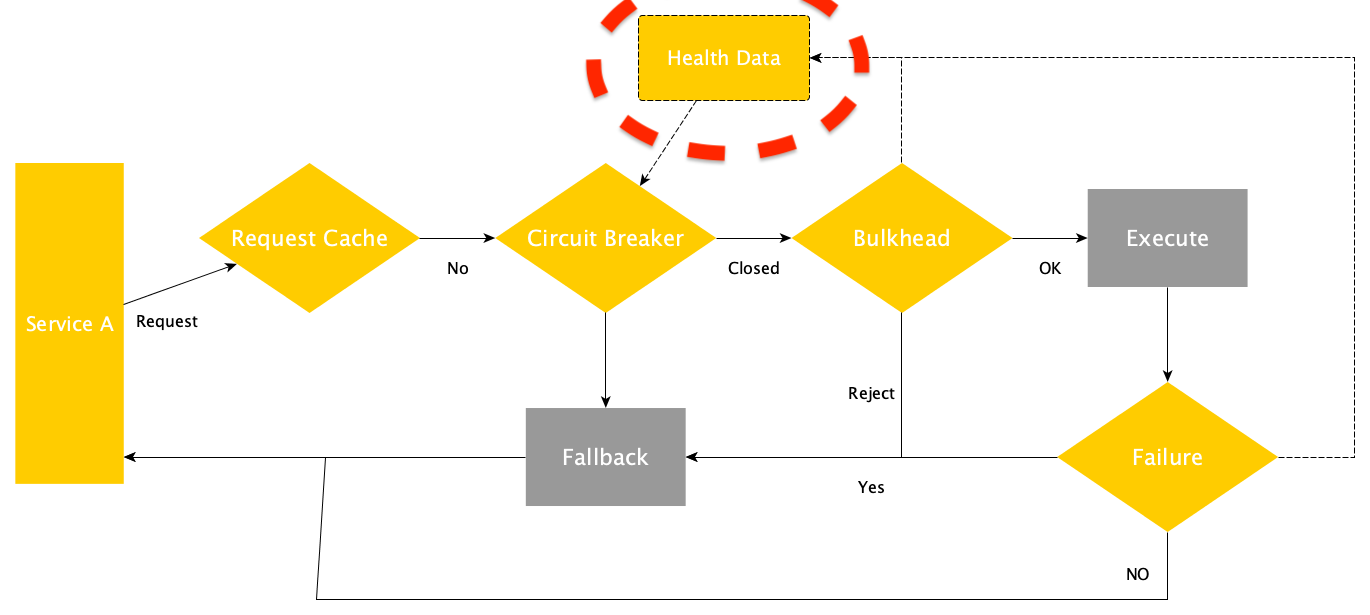
\includegraphics[width=\linewidth]{Images/falldata}
\end{figure}

\end{frame}

\begin{frame}[fragile]{Case 0.1 - Counted}
\begin{lstlisting}
@Inject
@Metric
Counter failedQueries;
\end{lstlisting}

\begin{lstlisting}
@GET
@Path("/{id:[a-z]*[0-9][0-9]*}")
@Fallback(fallbackMethod = "findByIdFallBack")
@Timeout(TIMEOUT)
public Response findById(@PathParam("id") 
final String imdbId) {
...
}

public Response findByIdFallBack(@PathParam("id") 
final String imdbId) {
...
}
\end{lstlisting}
\end{frame}

\begin{frame}[fragile]{Case 0.2 - Gauge}
Flat metric
\begin{lstlisting}
@Gauge(unit = "ExternalDatabases",
	name = "movieDatabases",
	absolute = true)
public long getDatabases() {
	return 1;
}
\end{lstlisting}

\lstinline|/metrics/application/movieDatabases|
\end{frame}

\begin{frame}[fragile]{Case 0.3 - Metered}
Measure of events rate
\begin{lstlisting}
@Metered(name = "moviesRetrieved",
	unit = MetricUnits.MINUTES,
	description = "Metrics to monitor movies",
	absolute = true)
public Response findExpandedById(@PathParam("id") final Long id) 
\end{lstlisting}

\lstinline|/metrics/application/movieDatabases|
\end{frame}

\begin{frame}[fragile]{Case 0.4 - Timed}
Measure of events delay and performance
\begin{lstlisting}
@Timed(name = "moviesDelay",
	description = "Metrics to monitor the times of movies retrieval",
	unit = MetricUnits.MINUTES,
	absolute = true)
public Response findExpandedById(@PathParam("id") final Long id) 
\end{lstlisting}

\lstinline|/metrics/application/moviesDelay|
\end{frame}

\begin{frame}[fragile]{Case 0.3 - Prometheus}
\begin{figure}
	\centering
	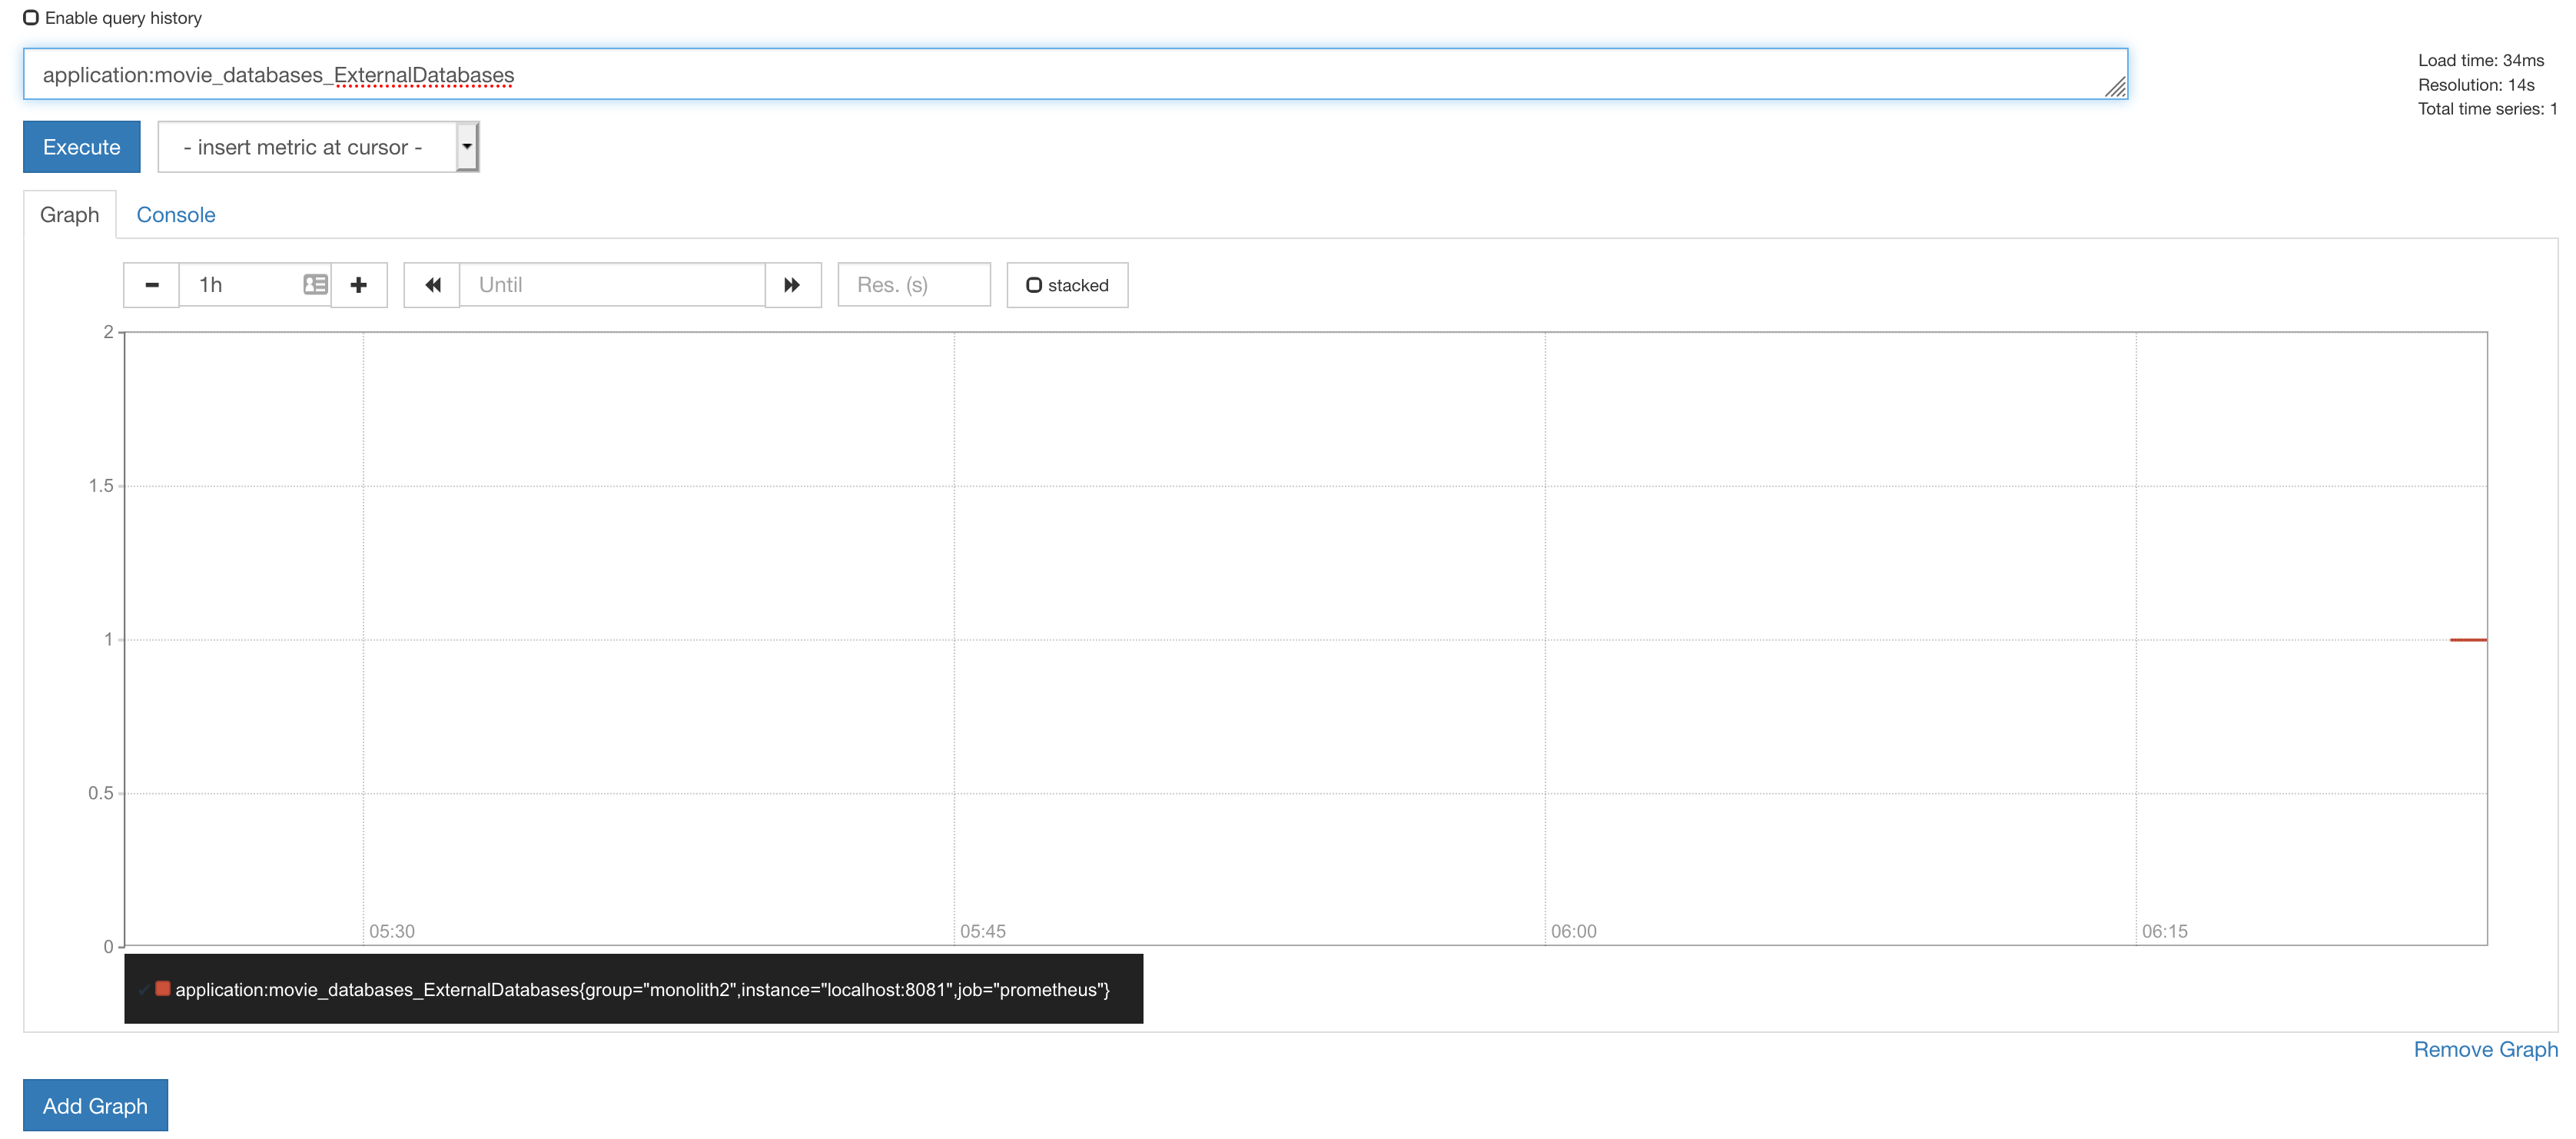
\includegraphics[width=\linewidth]{Images/gauge}
\end{figure}

\end{frame}

\begin{frame}{Case 1 - Application metrics}
\begin{figure}
	\centering
	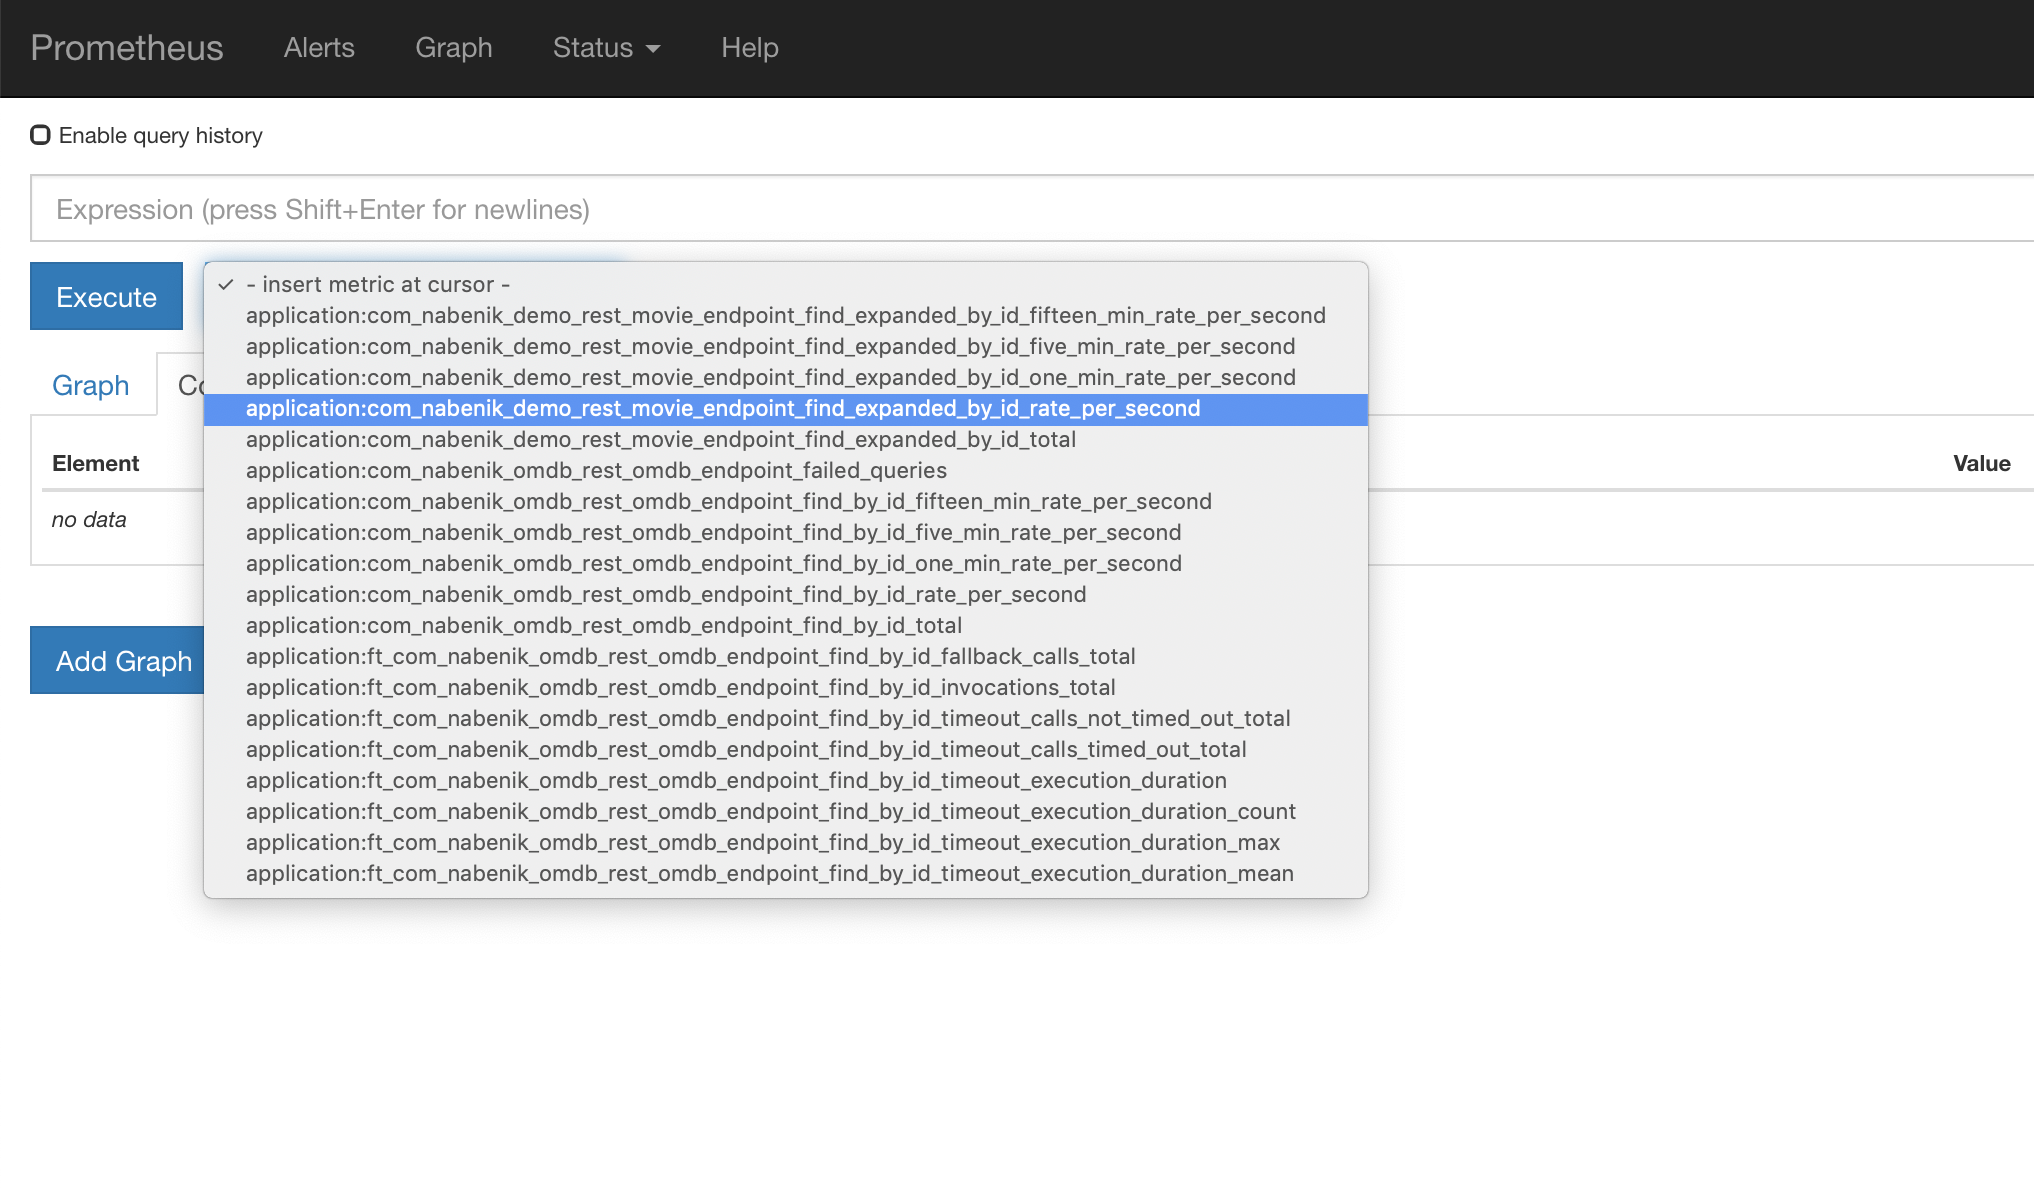
\includegraphics[width=\linewidth]{Images/micrometric1}
\end{figure}

\end{frame}

\begin{frame}{Case 1 - Counter over time}

\begin{figure}
	\centering
	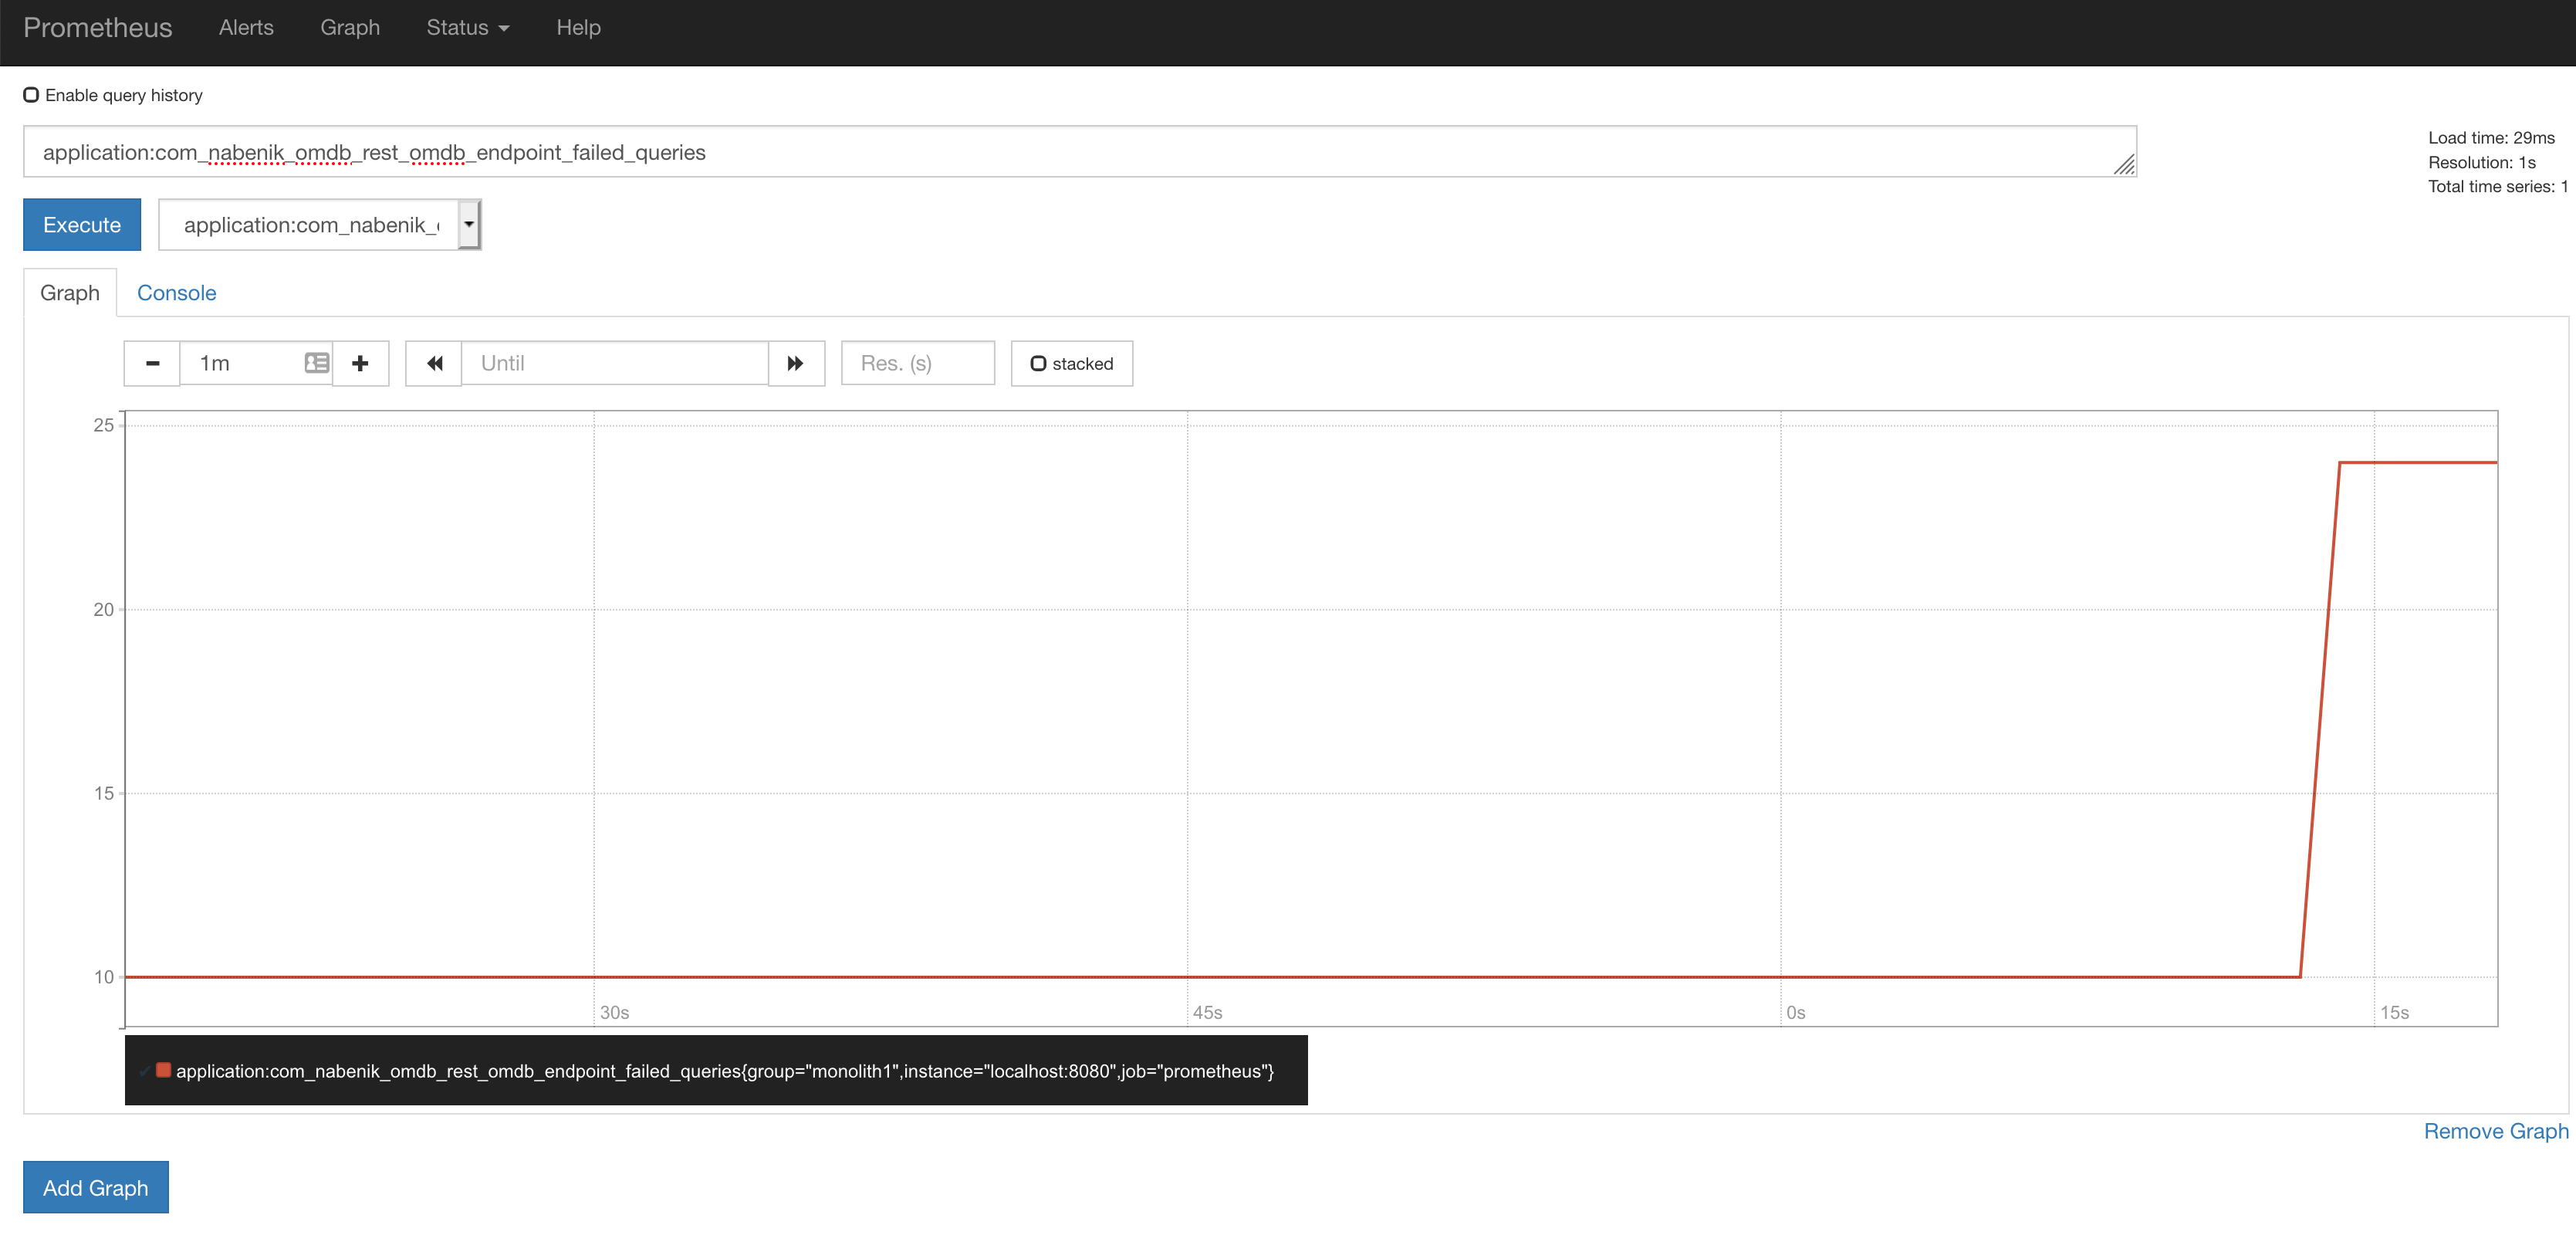
\includegraphics[width=\linewidth]{Images/micrometric2}
\end{figure}
\lstinline|application:com_nabenik_omdb_rest_omdb_endpoint_failed_queries|
\end{frame}



\begin{frame}{Case 1 - Telemetry for monoliths}

\begin{enumerate}
	\item Base metrics are almost JVM metrics
	\item JMX is also a pull-based monitoring technology
	\item Ideal for PaaS
\end{enumerate}

\begin{figure}
	\centering
	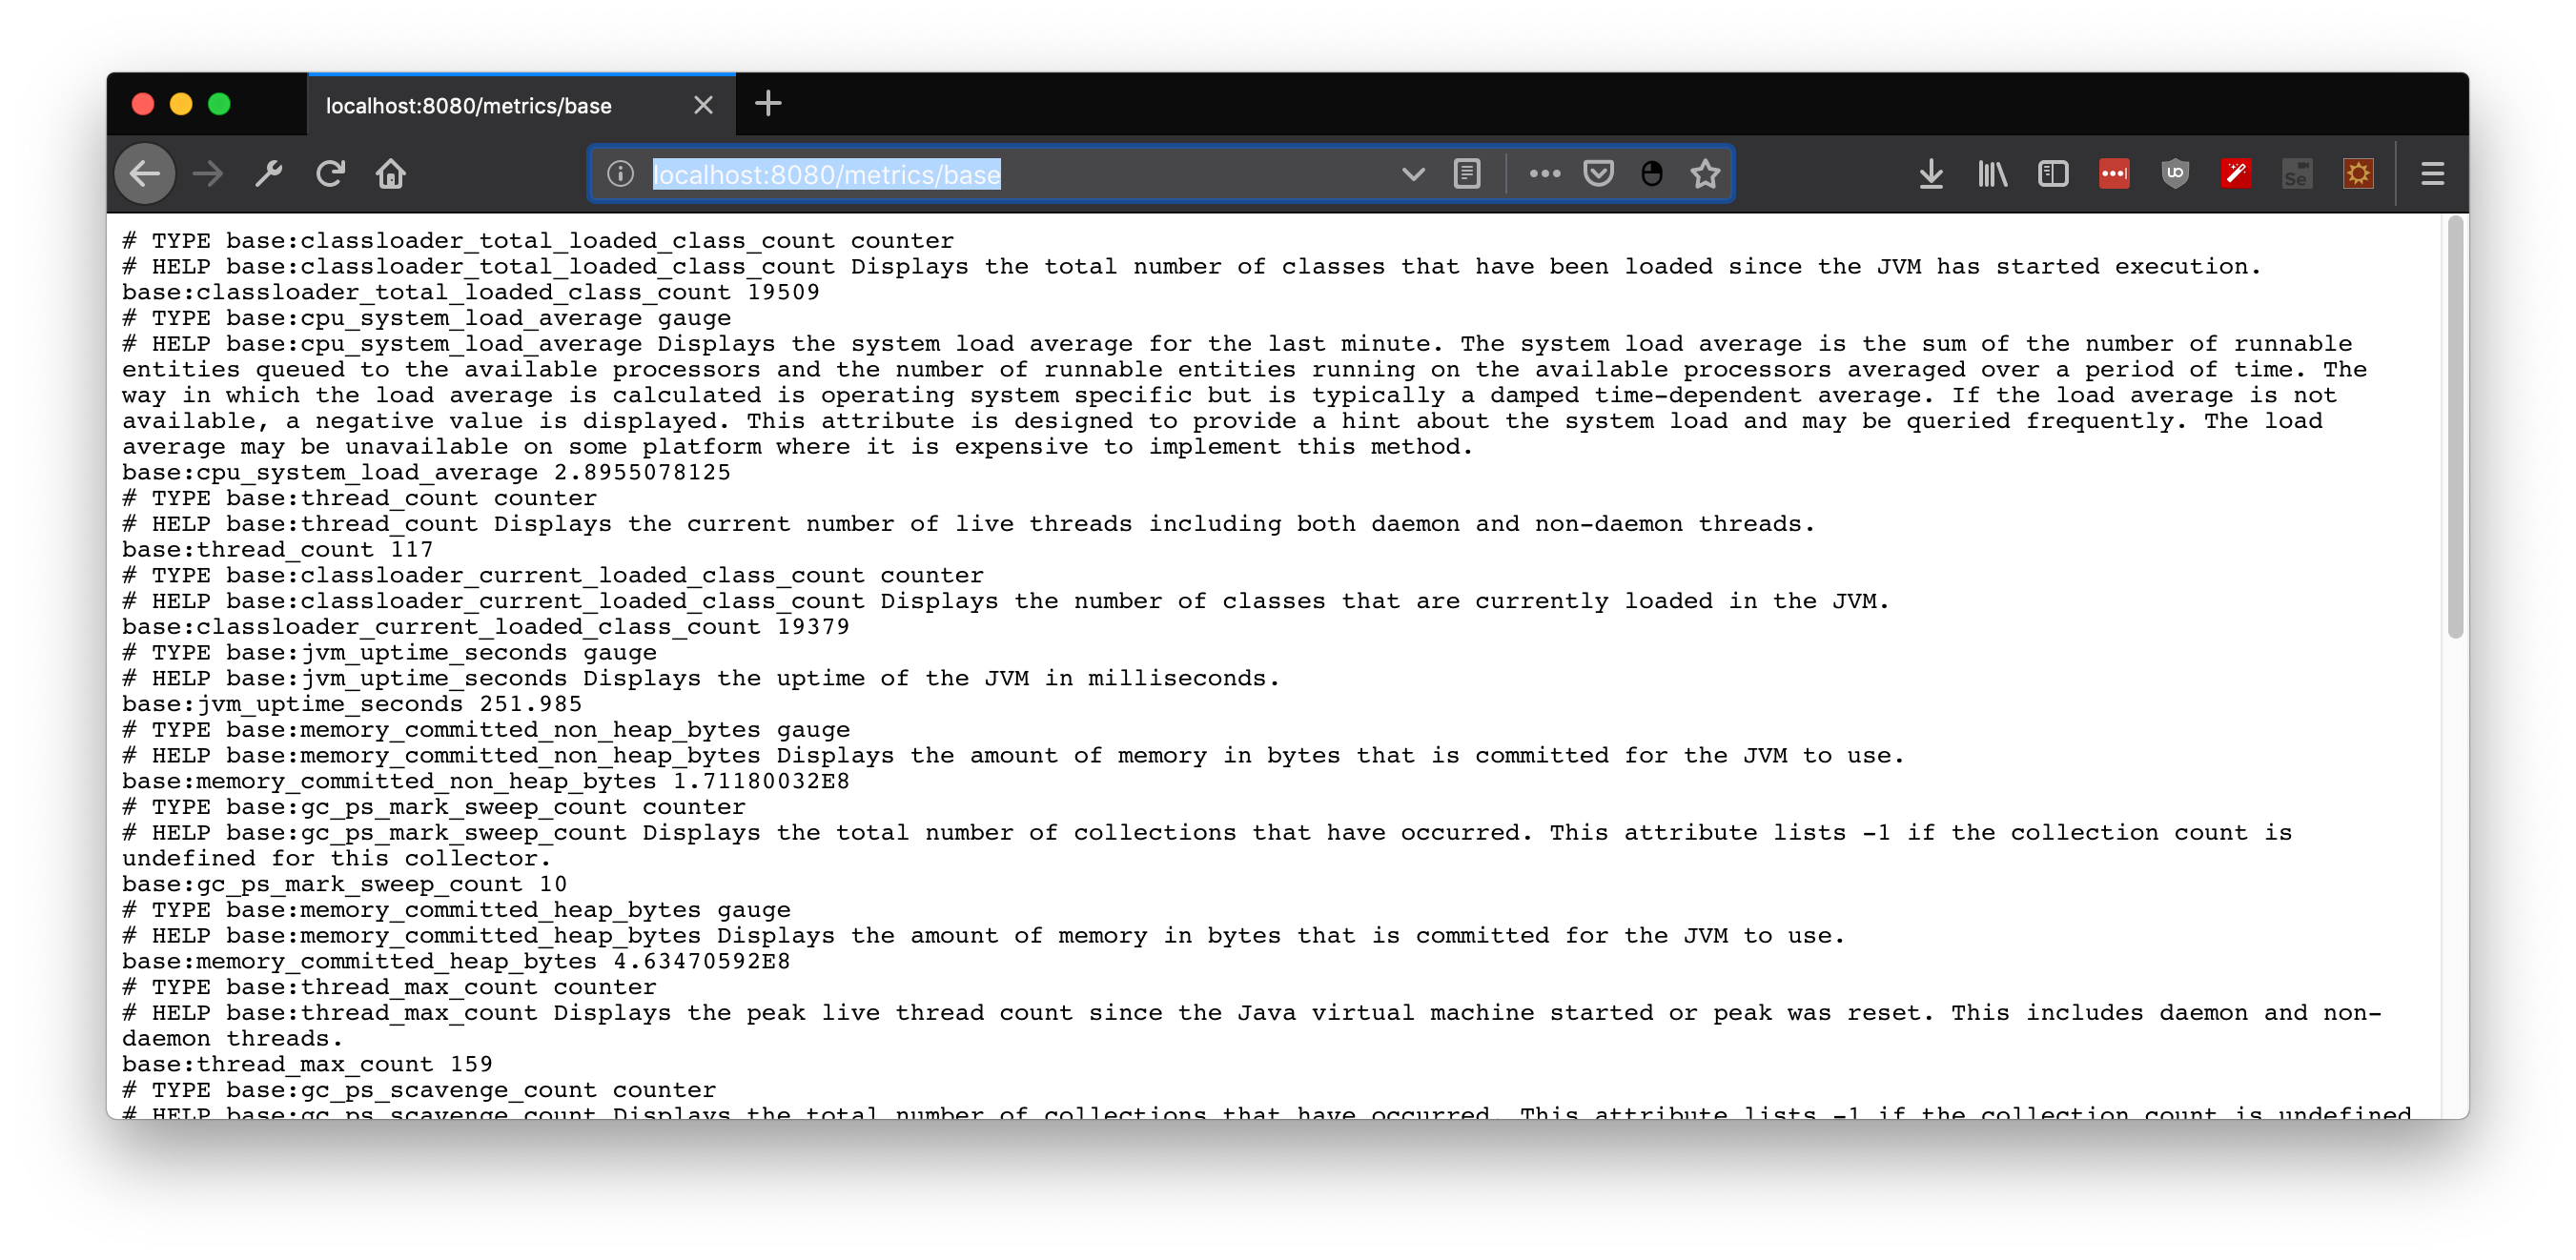
\includegraphics[width=\linewidth]{Images/base-metrics}
\end{figure}



\end{frame}

\begin{frame}{Case 1 - Heap performance}

\begin{figure}
	\centering
	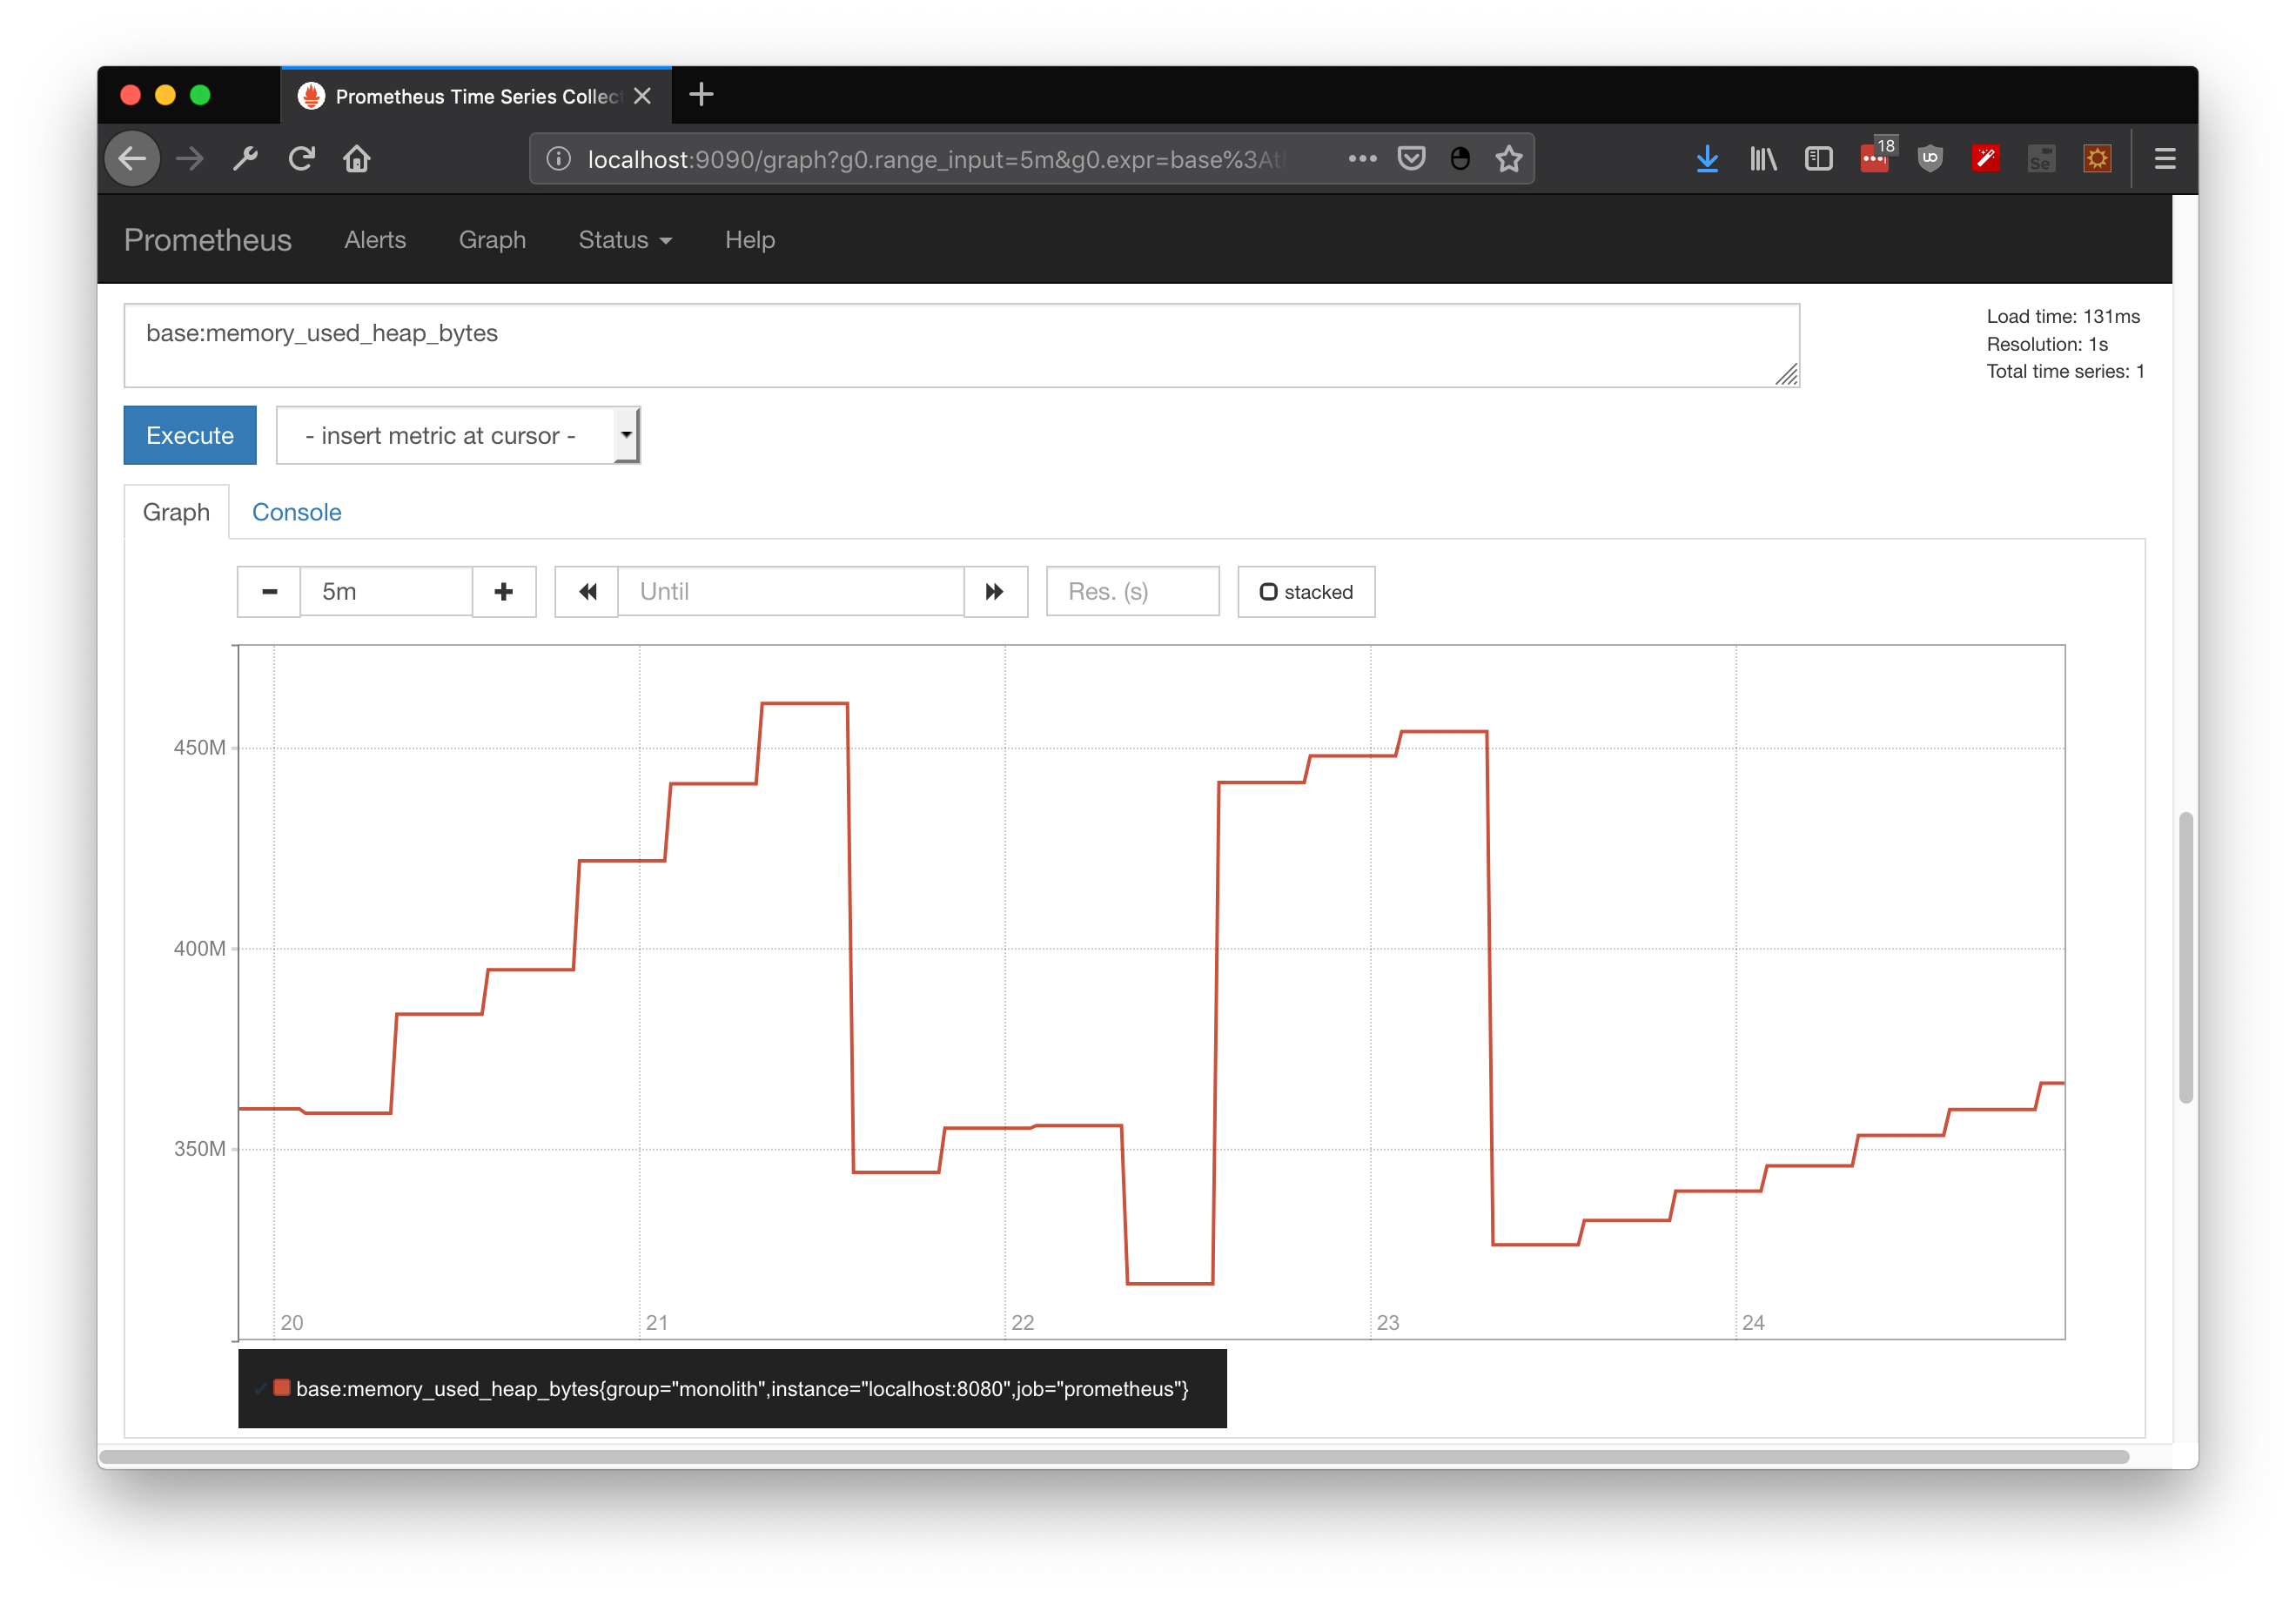
\includegraphics[width=0.8\linewidth]{Images/mono1}
\end{figure}
\lstinline|base:memory_used_heap_bytes|
\end{frame}

\begin{frame}{Case 1 - CPU Utilization}

\begin{figure}
	\centering
	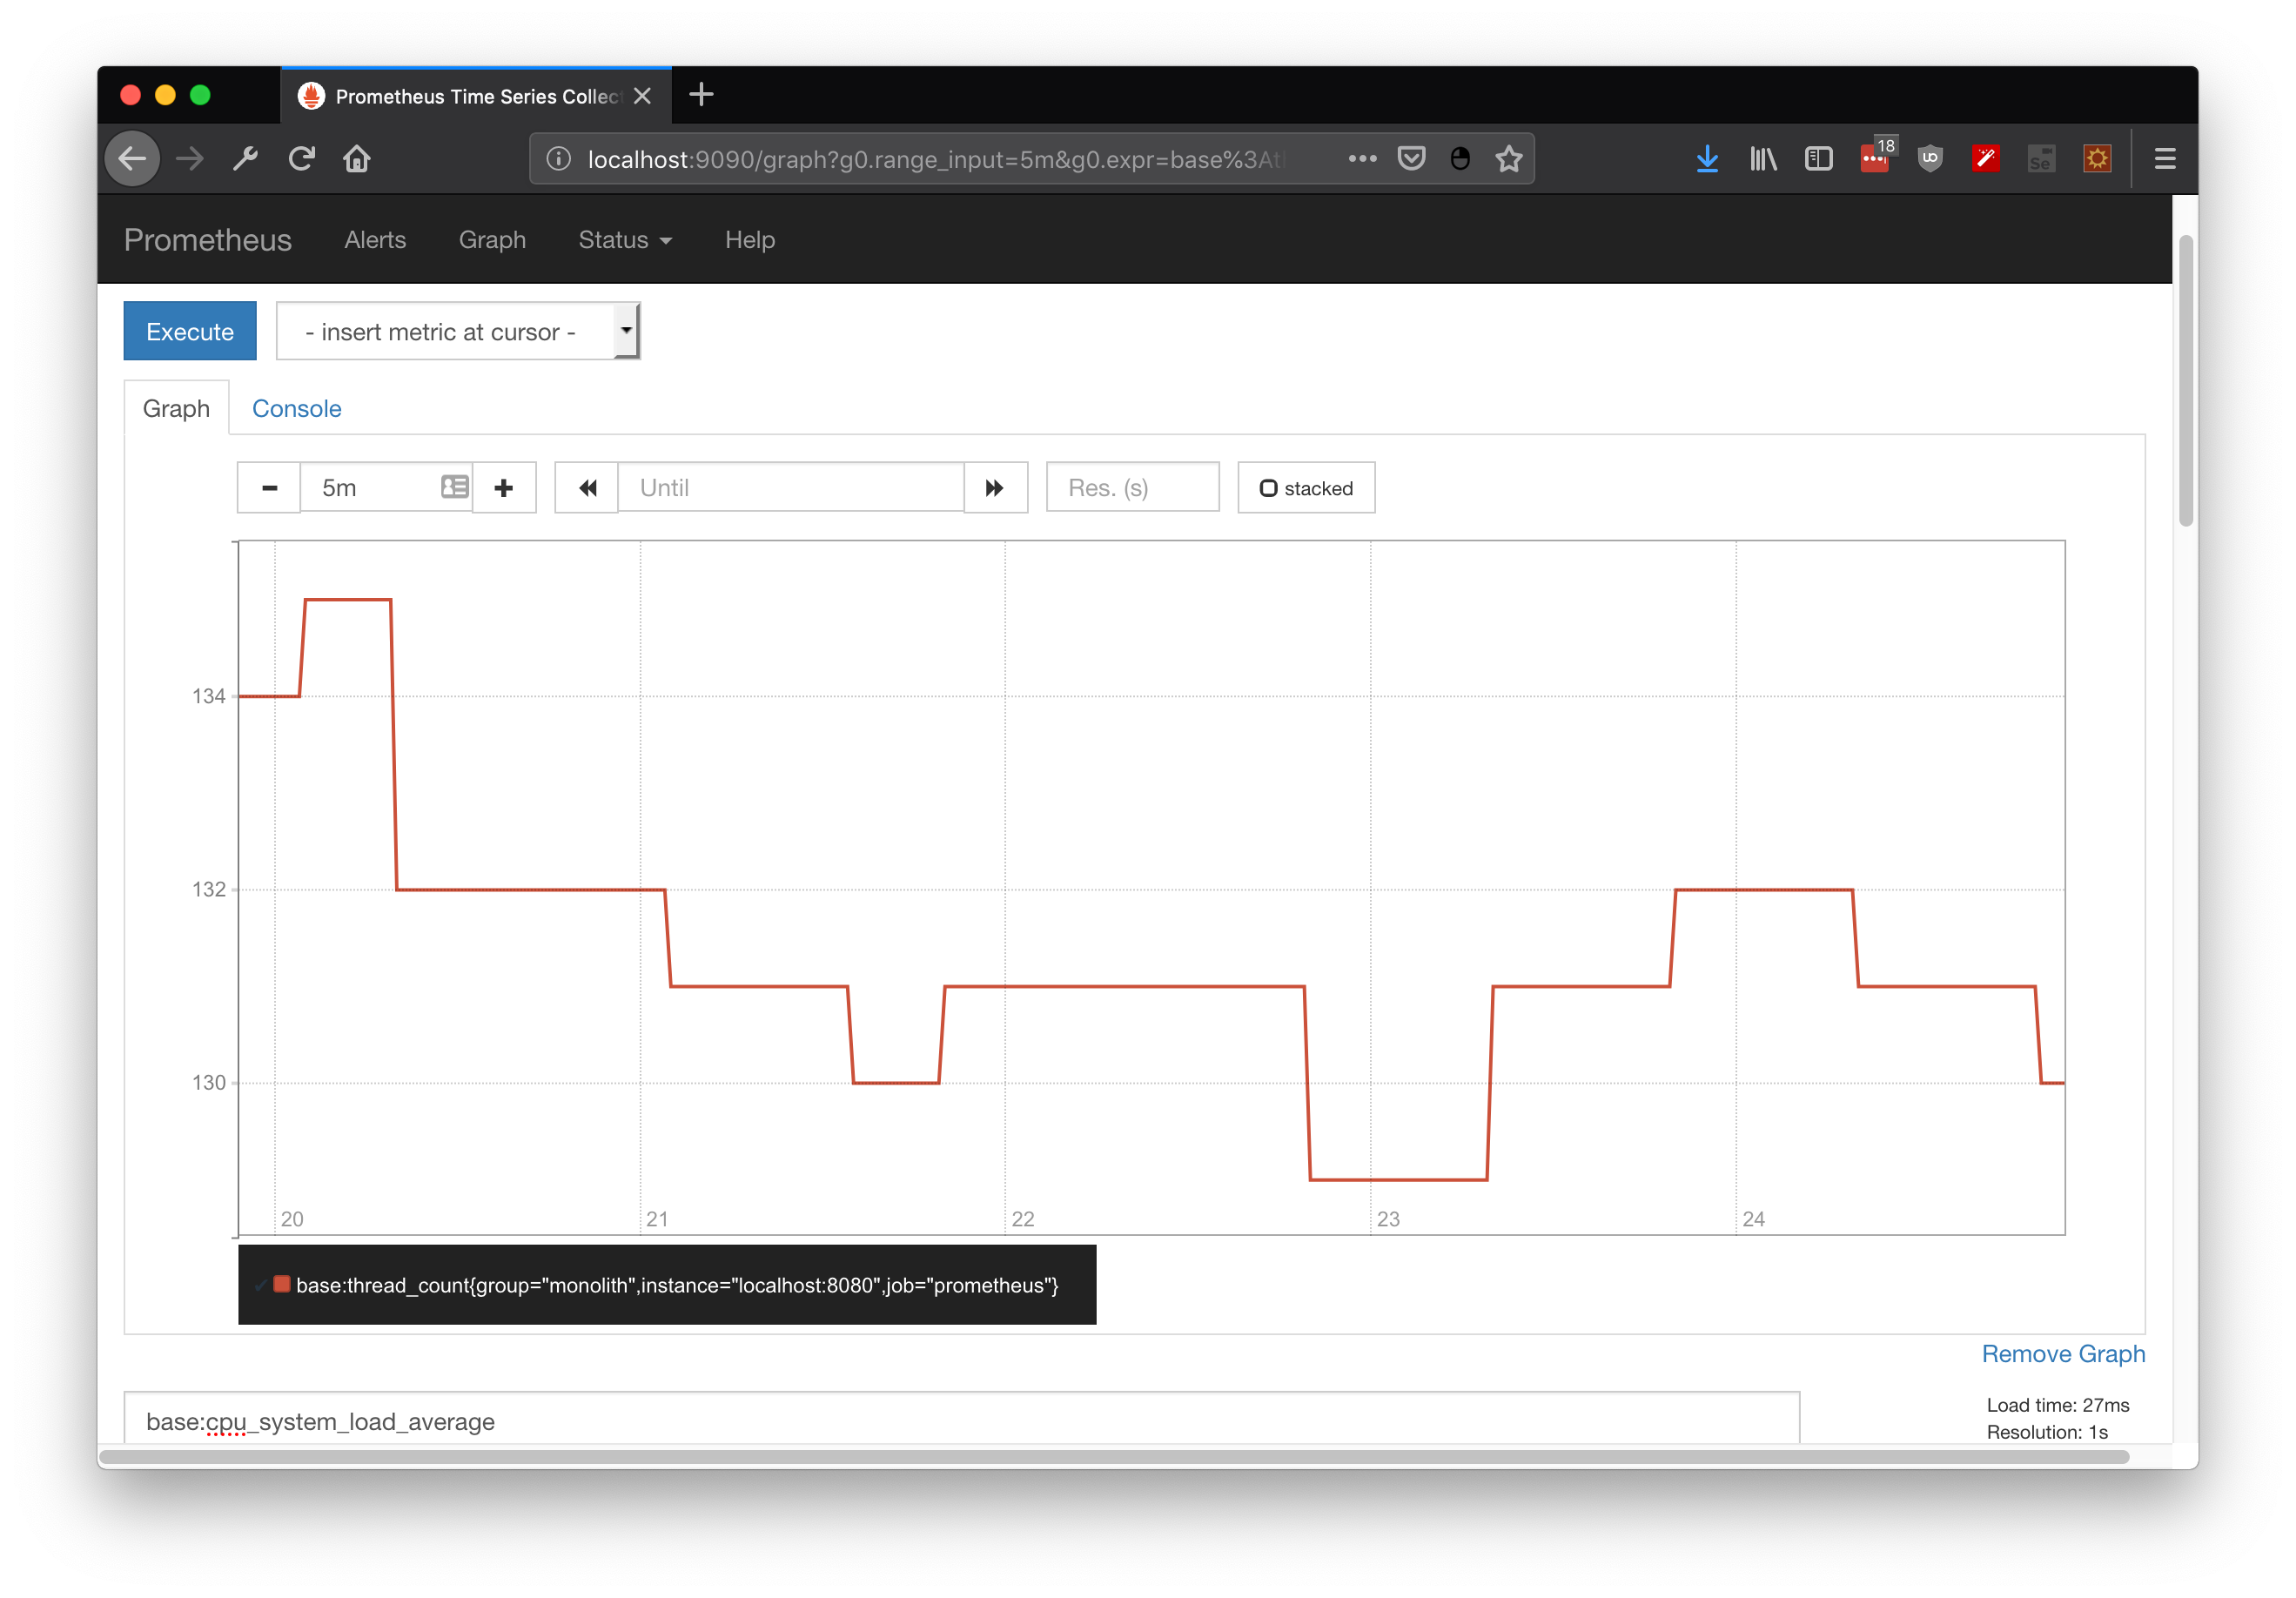
\includegraphics[width=0.8\linewidth]{Images/mono2}
\end{figure}
\lstinline|base:cpu_system_load_average|
\end{frame}

\begin{frame}{Case 1 - GC Executions}

\begin{figure}
	\centering
	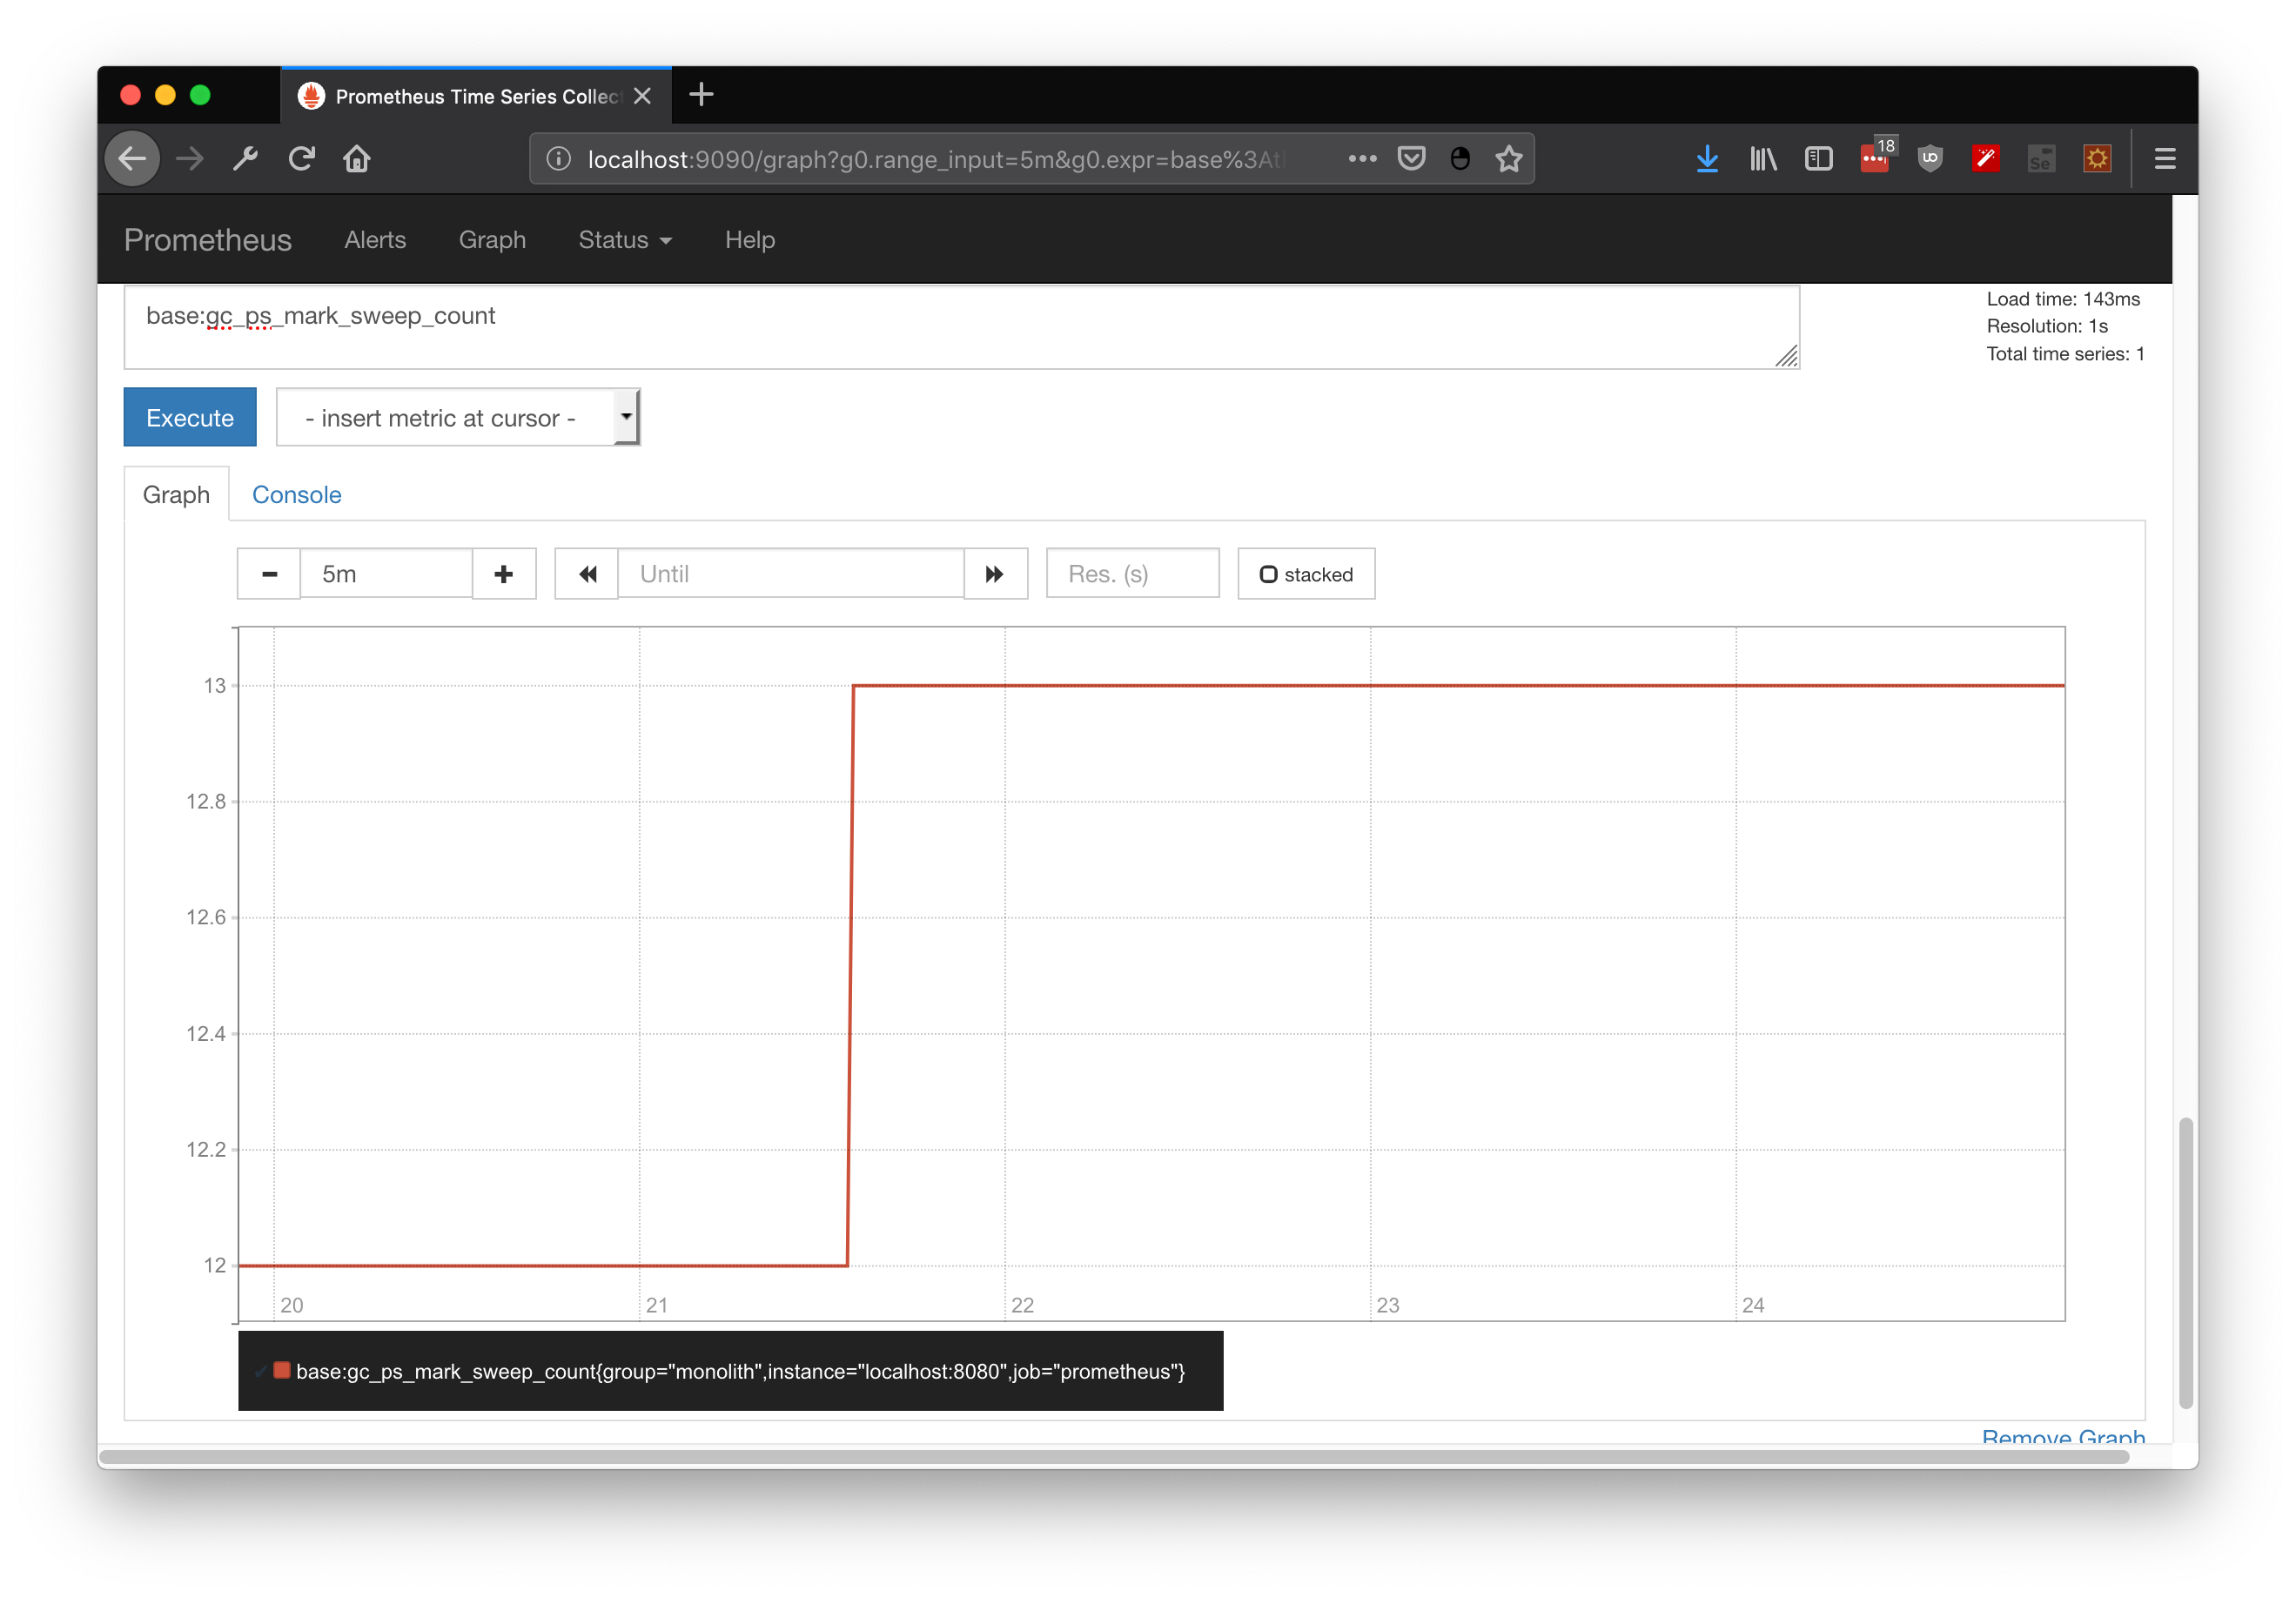
\includegraphics[width=0.8\linewidth]{Images/mono3}
\end{figure}
\lstinline|base:gc_ps_mark_sweep_count|
\end{frame}





\begin{frame}{Thank you}
\begin{itemize}
\item me@vorozco.com
\item http://vorozco.com
\item http://github.com/tuxtor/slides
\end{itemize}
\begin{center}

\includegraphics[width=0.1\linewidth]{Images/cclogo}
\\
This work is licensed under a Creative Commons Attribution-ShareAlike 3.0.
\end{center}
\end{frame}

\end{document}

